\chapter{Results and Analysis}
% screenshots of the results - positive and negative
\section{Latent Semantic Analysis}
We experiment with multiple values of matrix rank reduction and we find that as we reduce the rank of documents-tokens matrices, they become more dense. As we reduce the ranks, the distribution of  the learnt weights also change. 

\subsection{Full-rank matrices}

Figure 13 shows the the similarity matrices computed using full-rank documents-tokens matrices for name and description and help text. We do not apply rank reduction on documents-tokens matrix of input and output file types. Using these similarity matrices, we find an optimal combination by optimizing them. The "optimal" correlation plot shows this weighted average. Figure 14 shows the distribution of weights for multiple tool attributes. We see the magnitude of weights learnt for input and output file types is higher than the other two. It is associated with the higher values captured for the similarity matrix of input and output file types.

\begin{figure}[h]
\begin{centering}
    {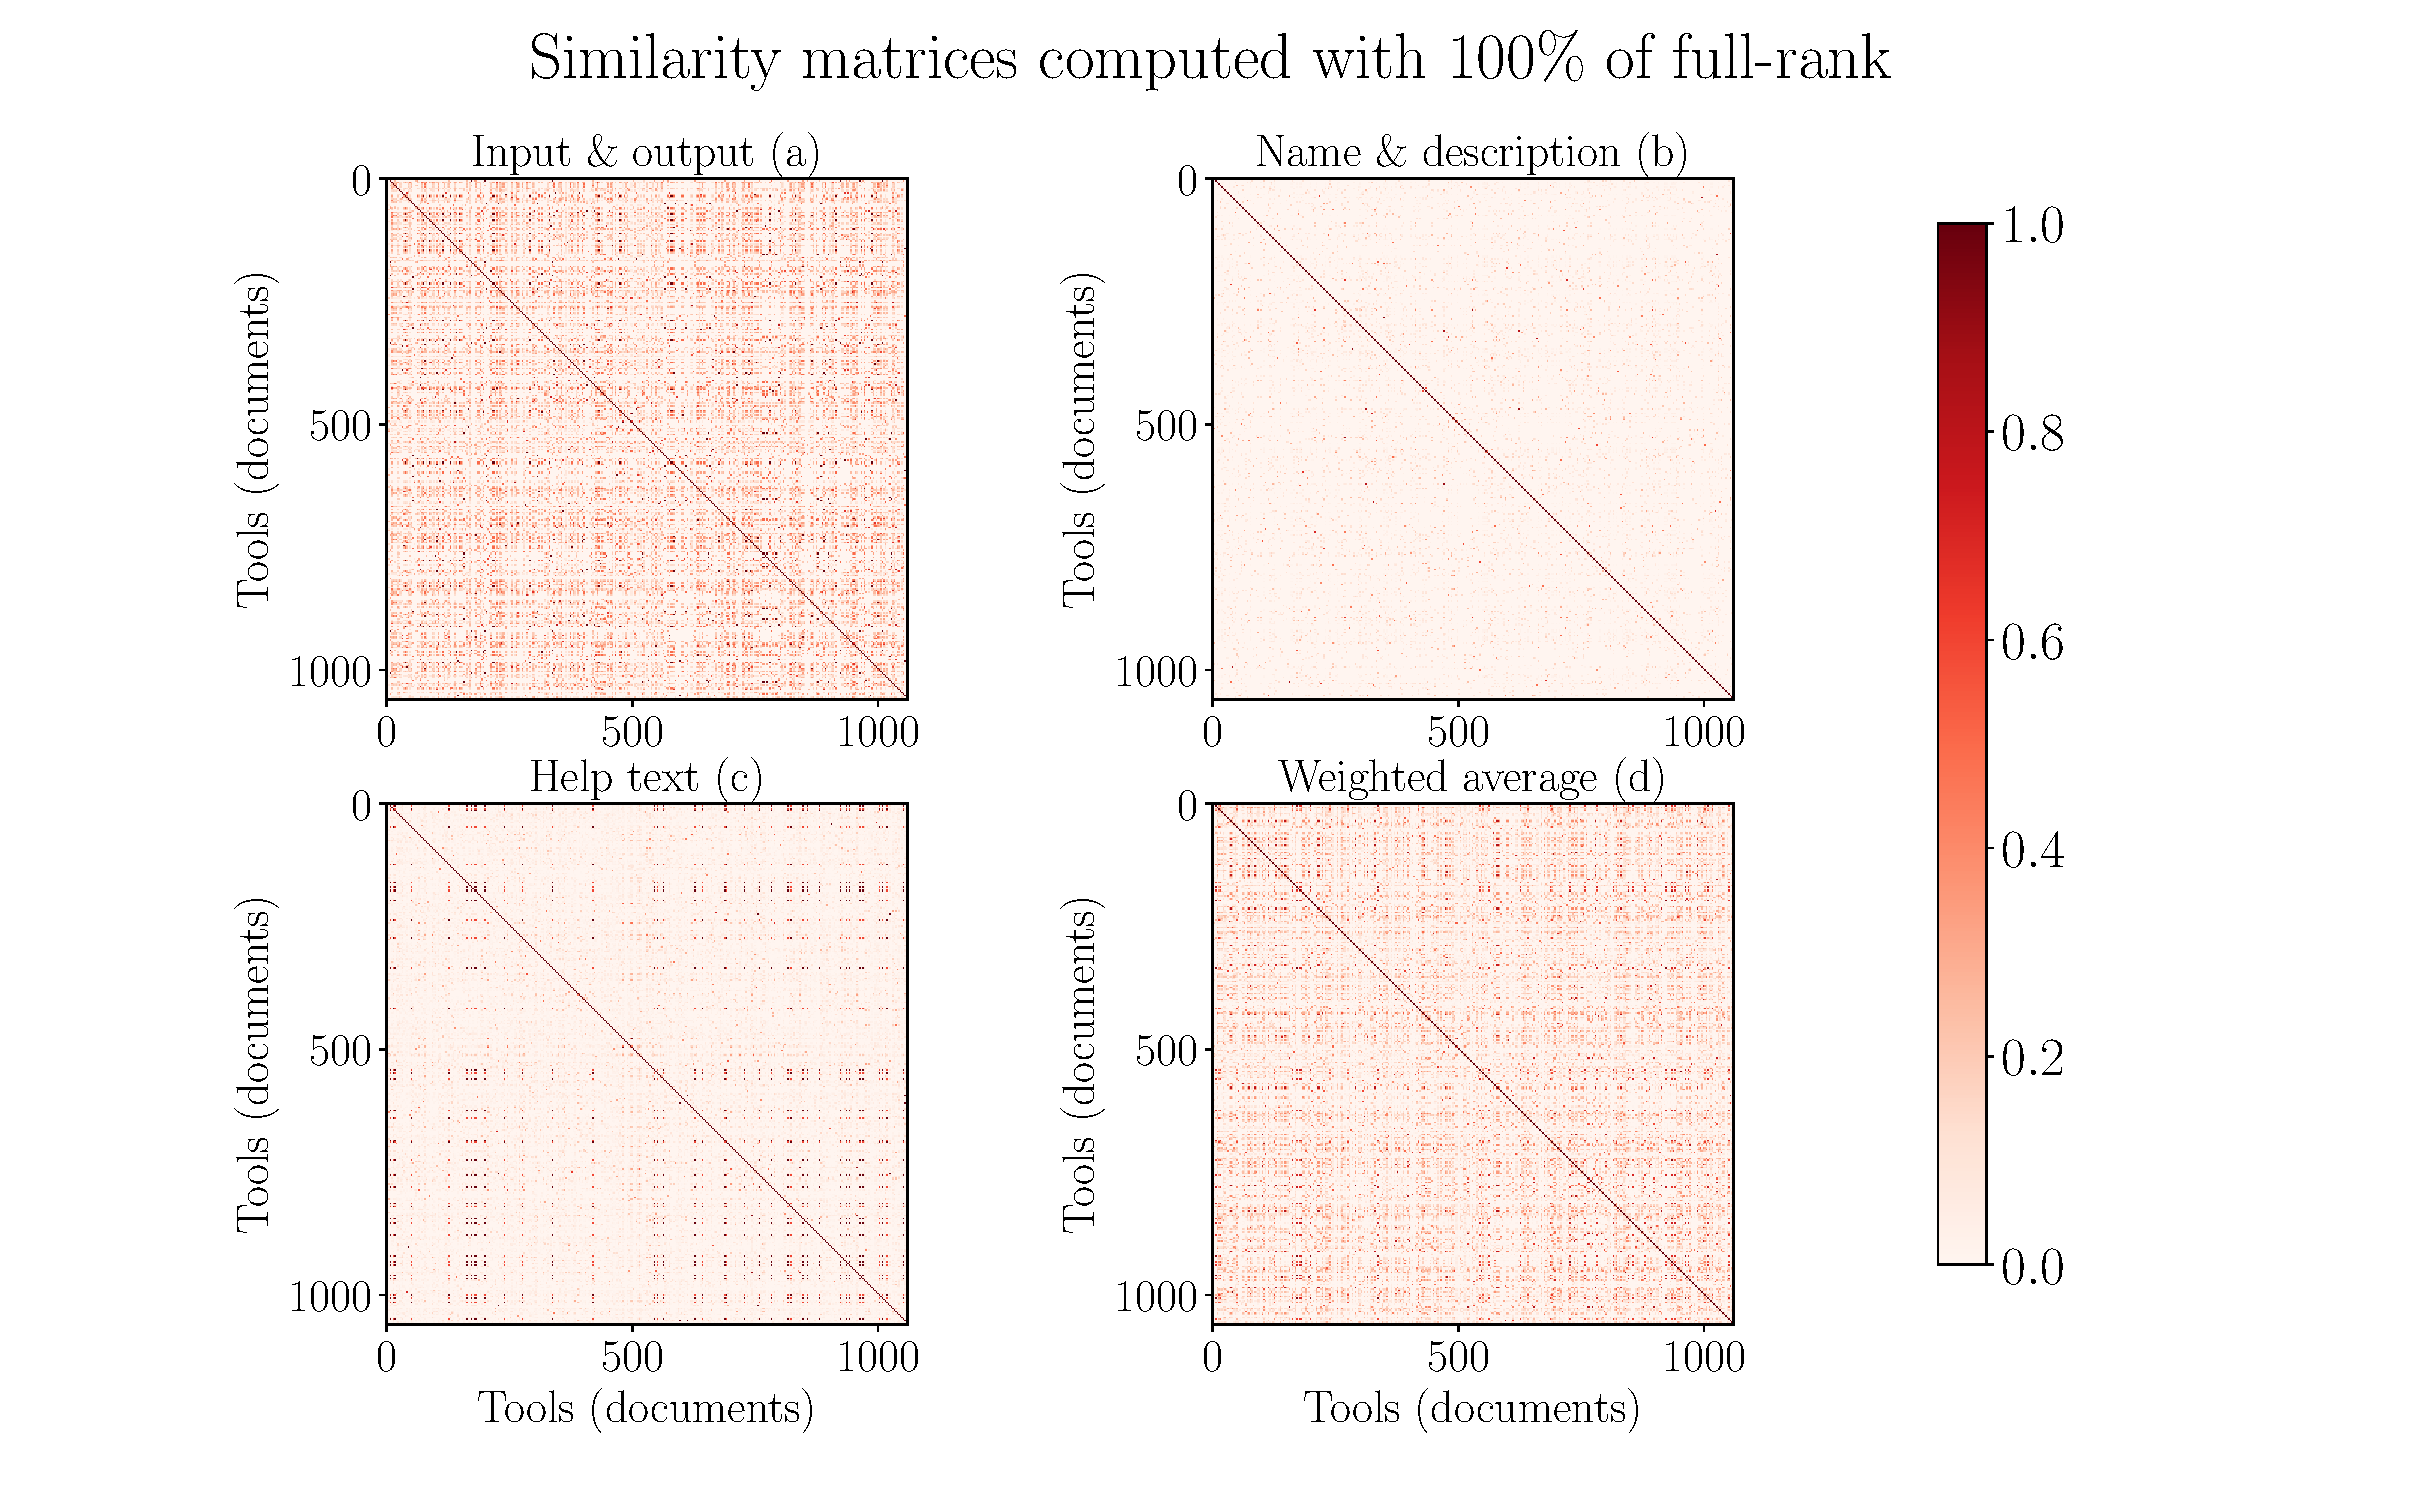
\includegraphics[scale=0.35]{figures/Similarity_matrices_100.pdf}}
    \caption[Similarity matrices full rank]{\textbf{Similarity matrices using full-rank}: The heatmap shows documents-documents (tools-tools) correlation matrices for input and output (a), name and description (b) and help text (c) attributes. The (d) shows a documents-documents (tools-tools) correlation matrix which is the weighted average computed using (a), (b) and (c) and weights (figure 18) given by the gradient descent optimizer (equation 15). The corresponding documents-tokens matrices contain their full-ranks. }
\end{centering}
\end{figure}

\begin{figure}[h]
\begin{centering}
    {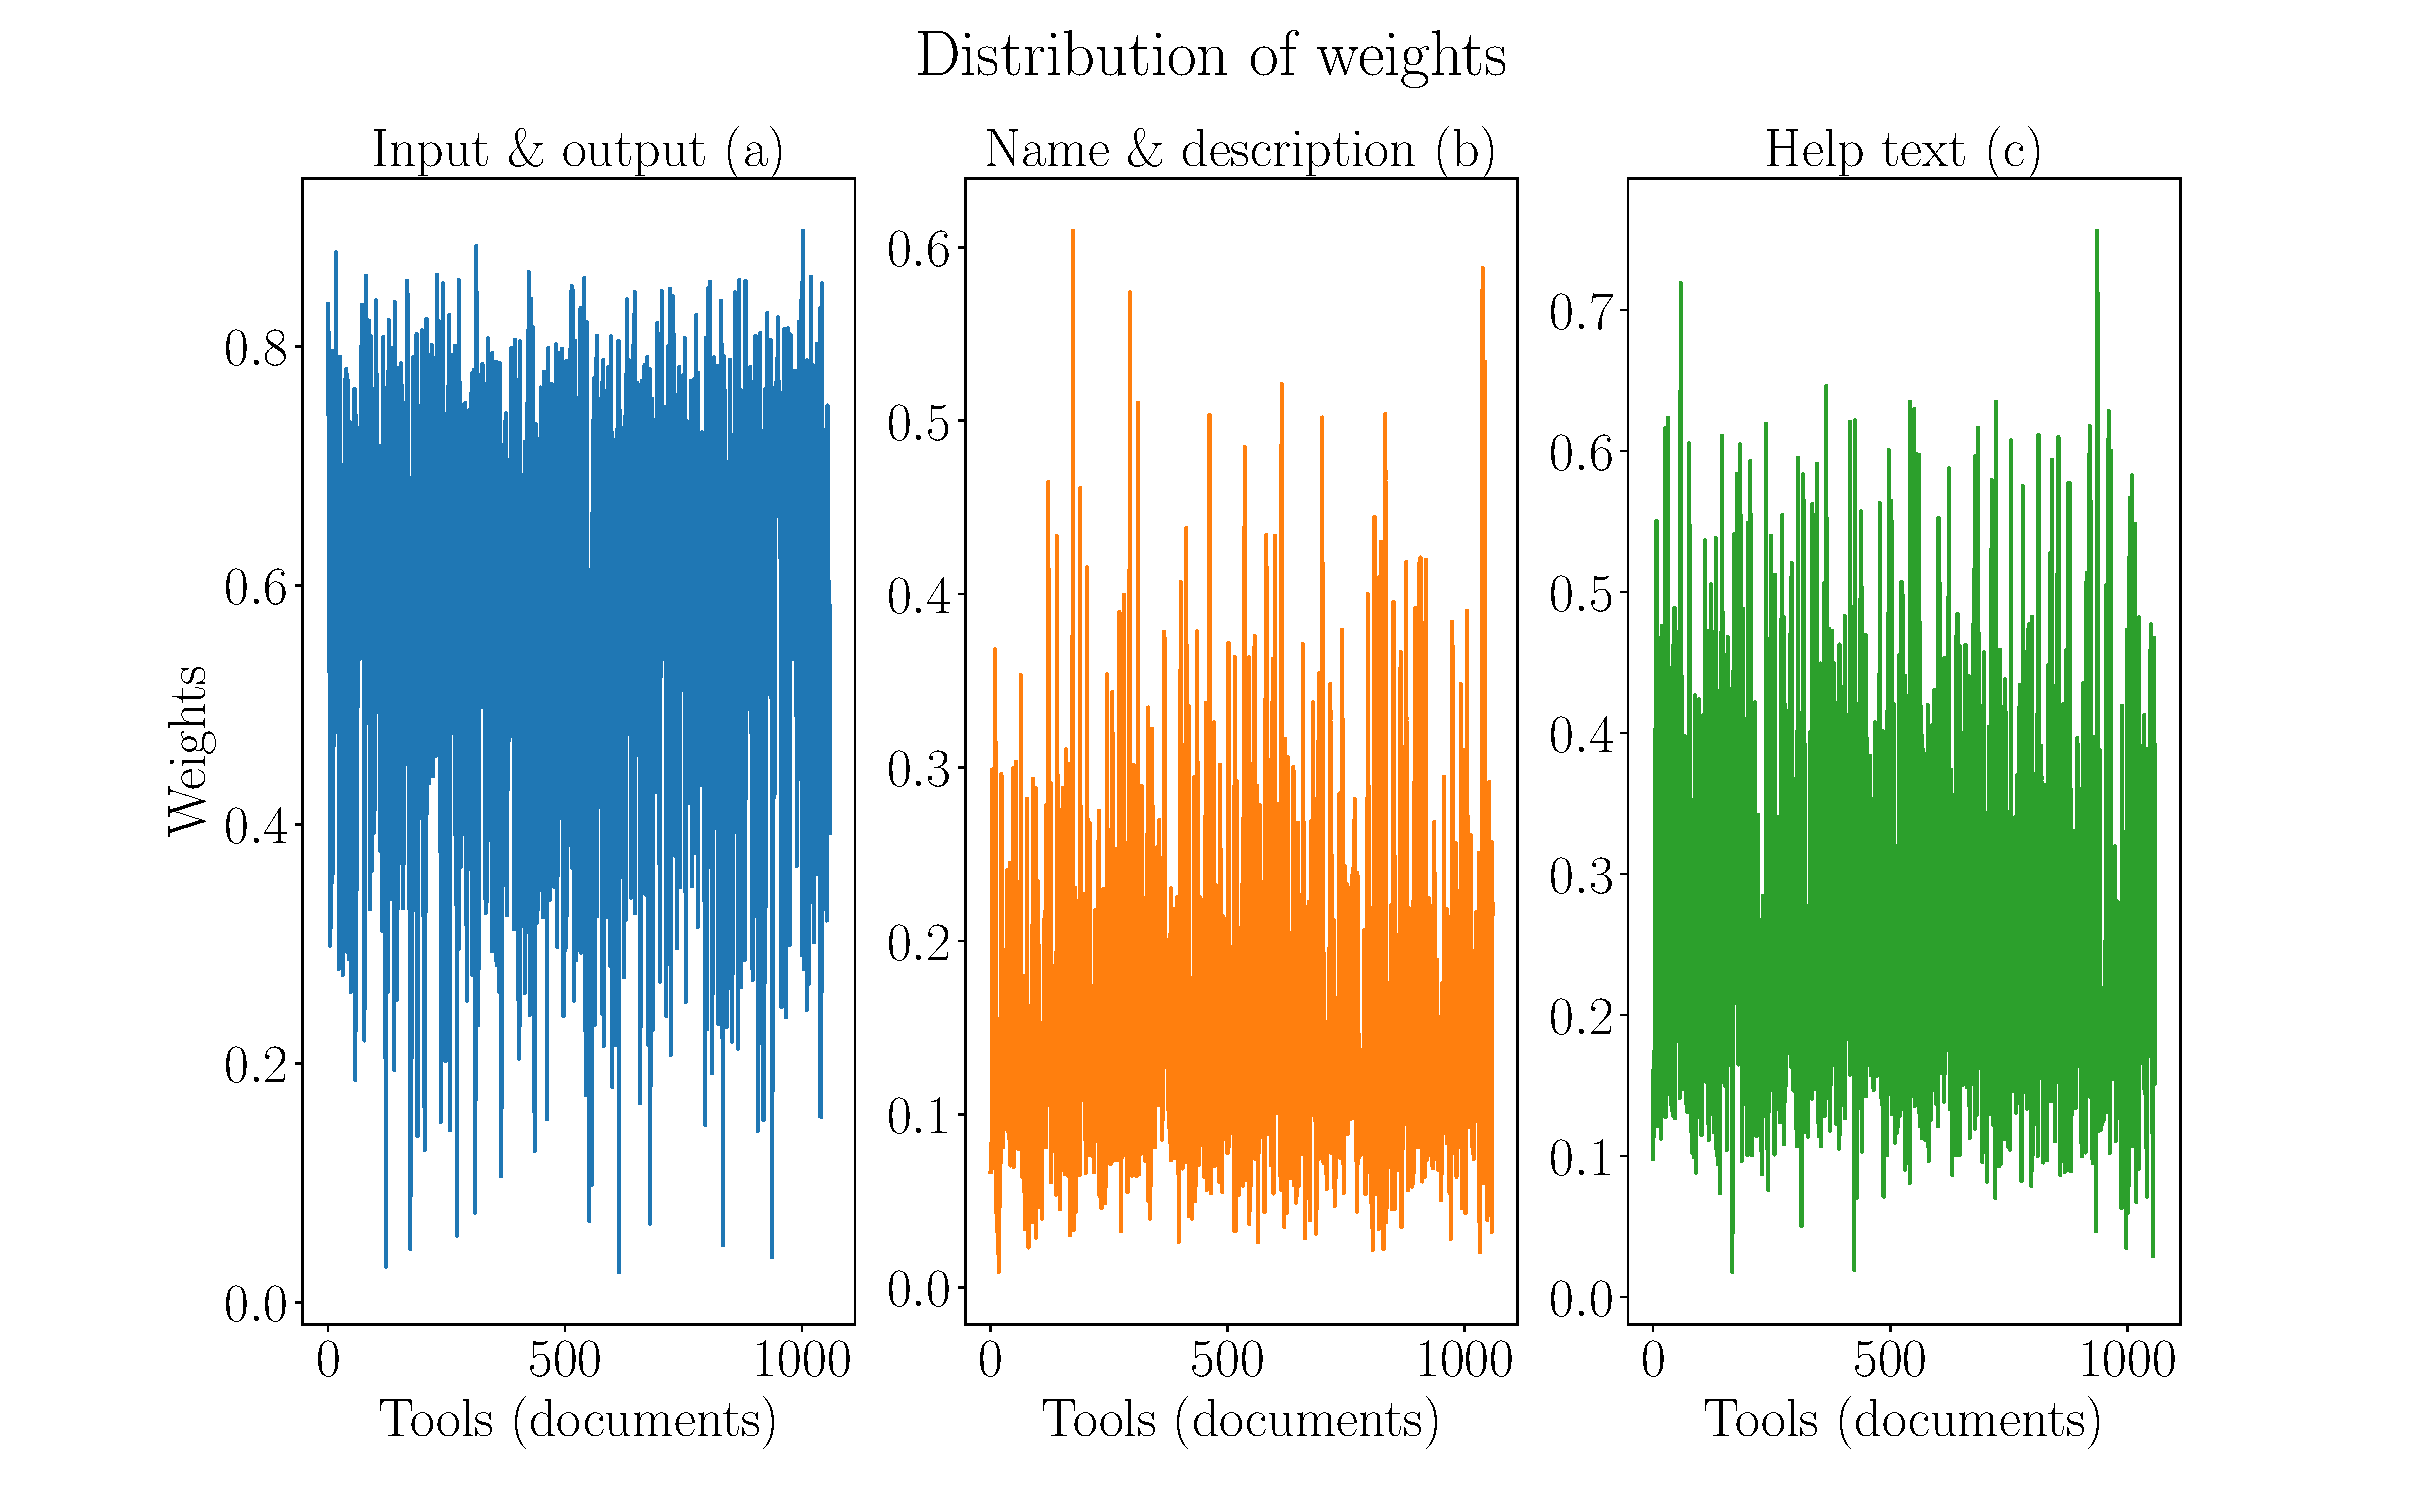
\includegraphics[scale=0.35]{figures/Weights_100.pdf}}
    \caption[Weights distribution full-rank]{\textbf{Weights distribution full- rank}: The plot shows the distribution of weights learned by gradient descent optimizer on the similarity matrices for the input and output, name and description and help text attributes. The corresponding documents-tokens matrices contain their full-ranks.}
\end{centering}
\end{figure}

\subsection{70\% of full-rank}
We reduce the ranks of two documents-tokens matrices to 70\% of full-rank. For example, if the rank of a matrix is 100, we reduce the rank to 70 using singular value decomposition. From figure 15, we see that the name and description and help text similarity matrices start becoming more dense compared to figure 13. The distribution of the weights also change (figure 16).

\begin{figure}[h]
\begin{centering}
    {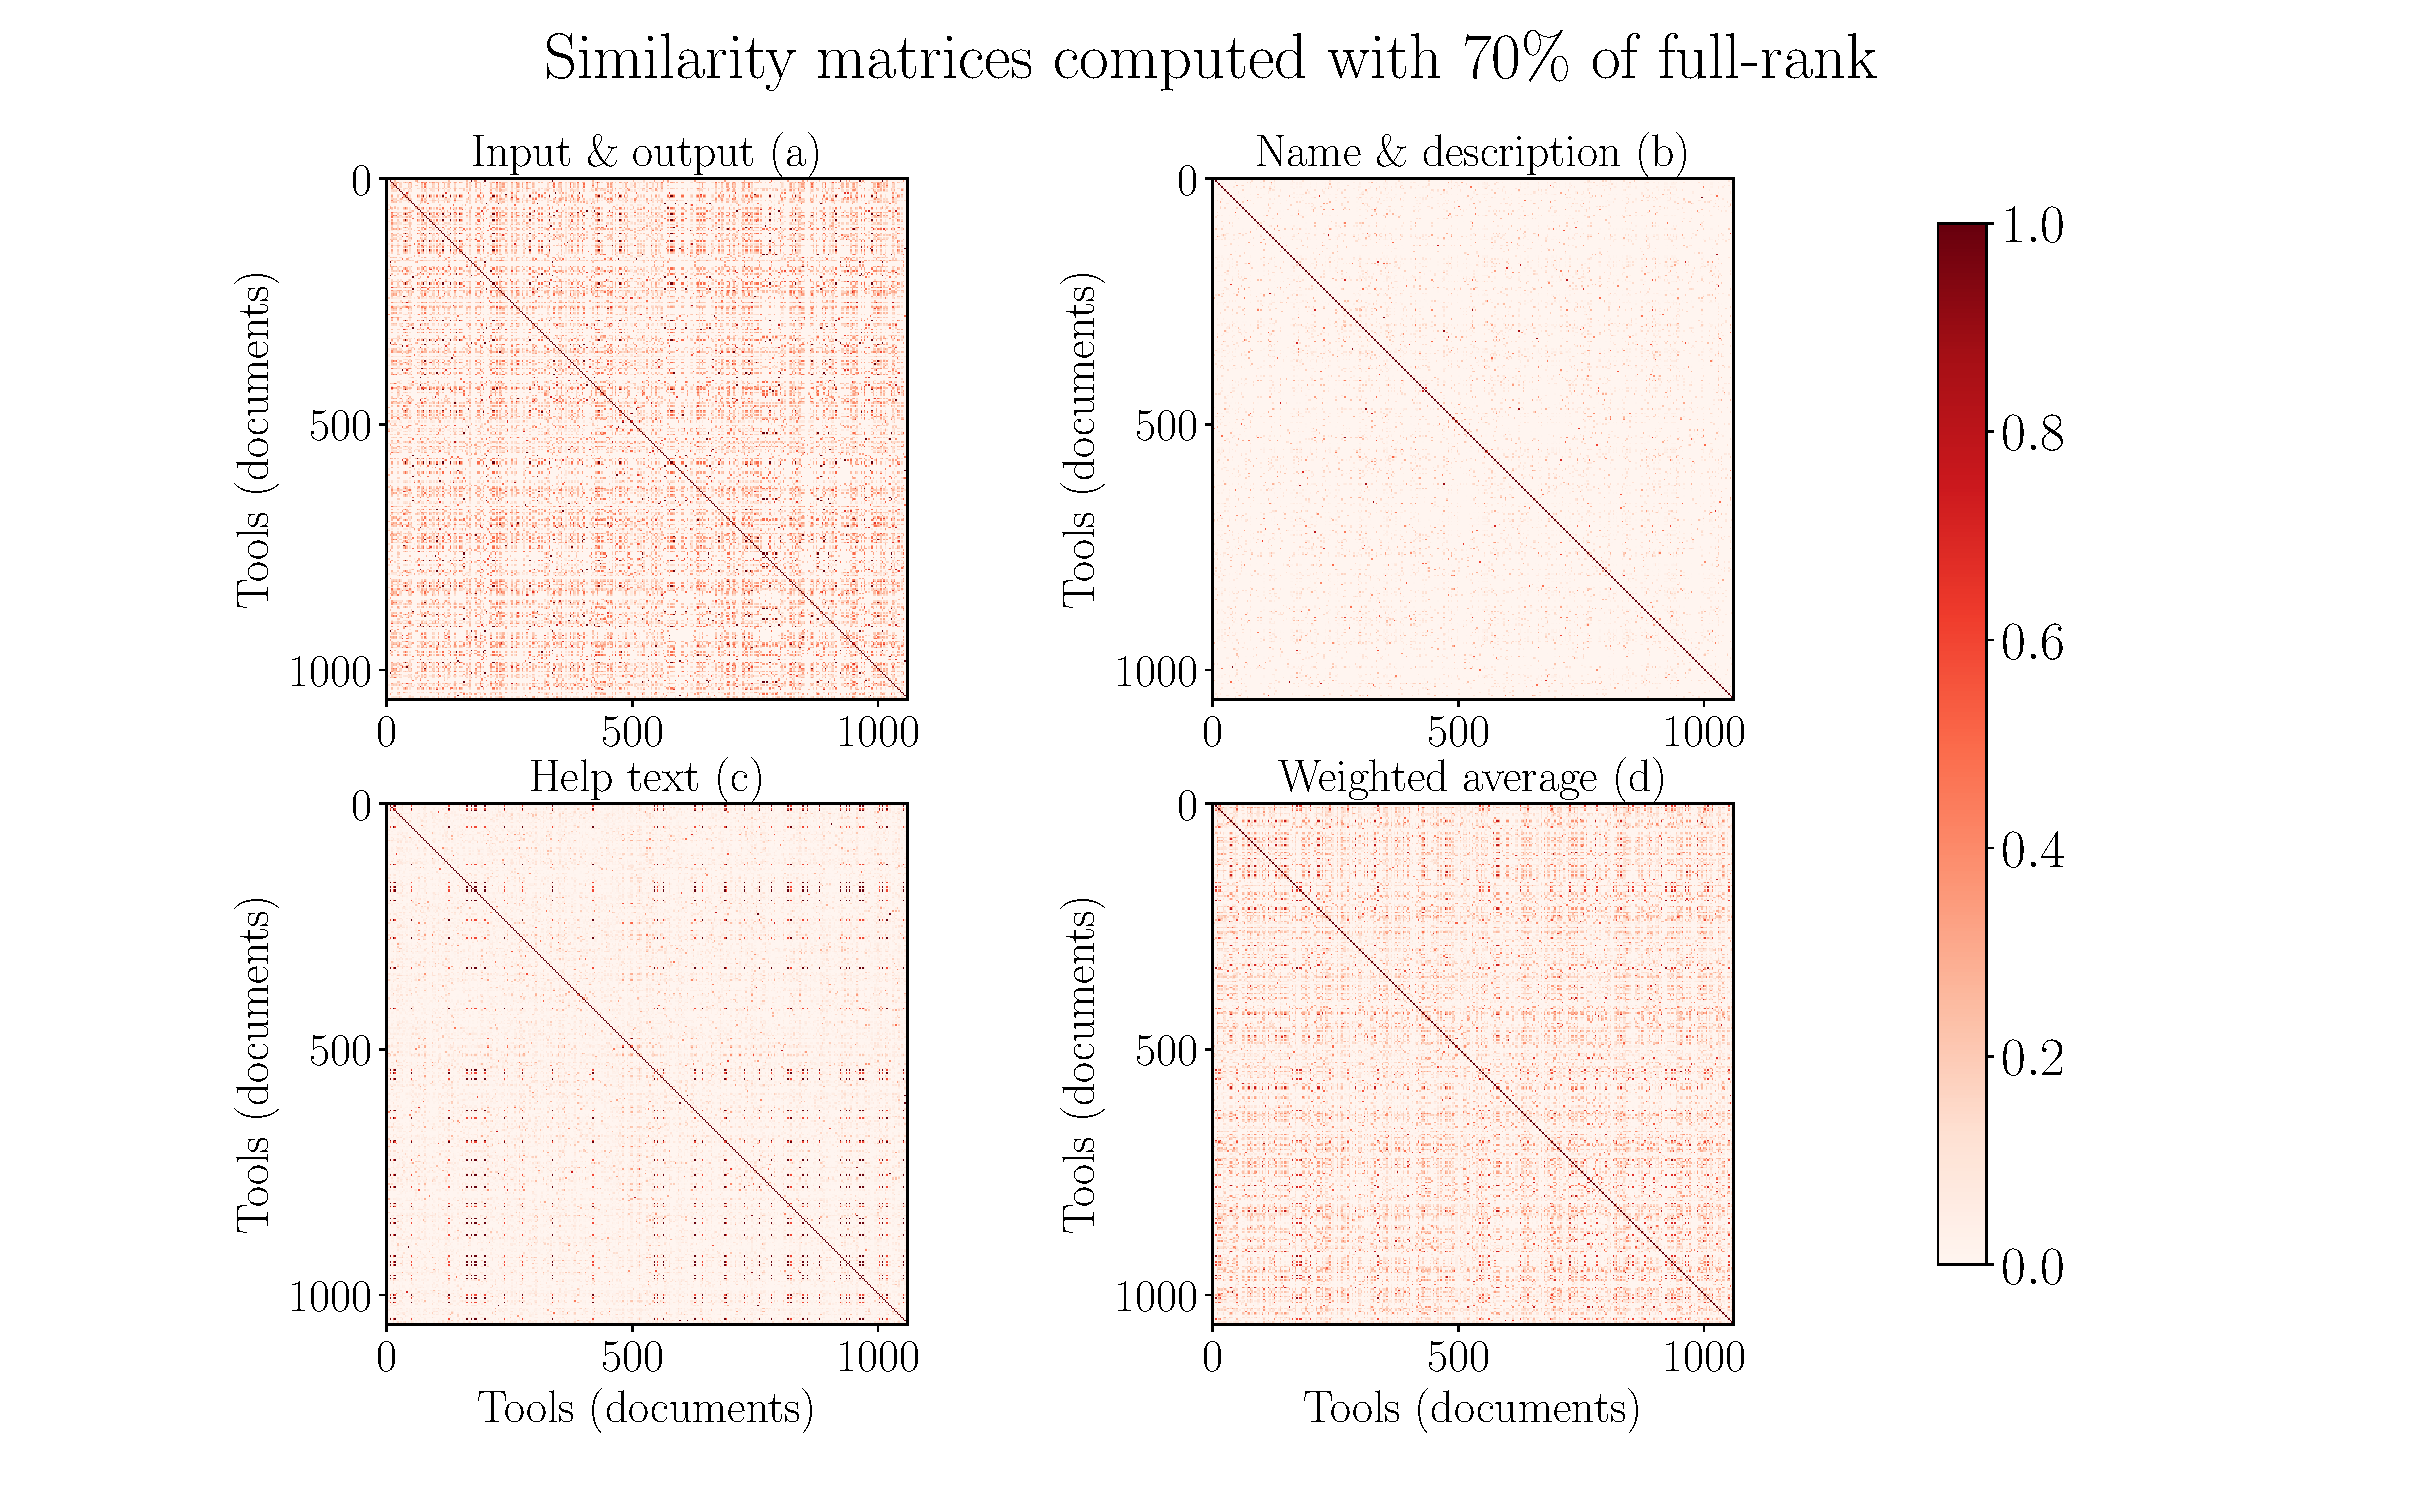
\includegraphics[scale=0.35]{figures/Similarity_matrices_070.pdf}}
    \caption[Similarity matrices 70\% rank]{\textbf{Similarity matrices using 70\% of full-rank}: The heatmap shows documents-documents (tools-tools) correlation matrices for input and output (a), name and description (b) and help text (c) attributes. The (d) shows a documents-documents (tools-tools) correlation matrix which is the weighted average computed using (a), (b) and (c) and weights (figure 20) given by the gradient descent optimizer (equation 15). The corresponding documents-tokens matrices are reduced to 70\% of their respective full-ranks.}
\end{centering}
\end{figure}

\begin{figure}[h]
\begin{centering}
    {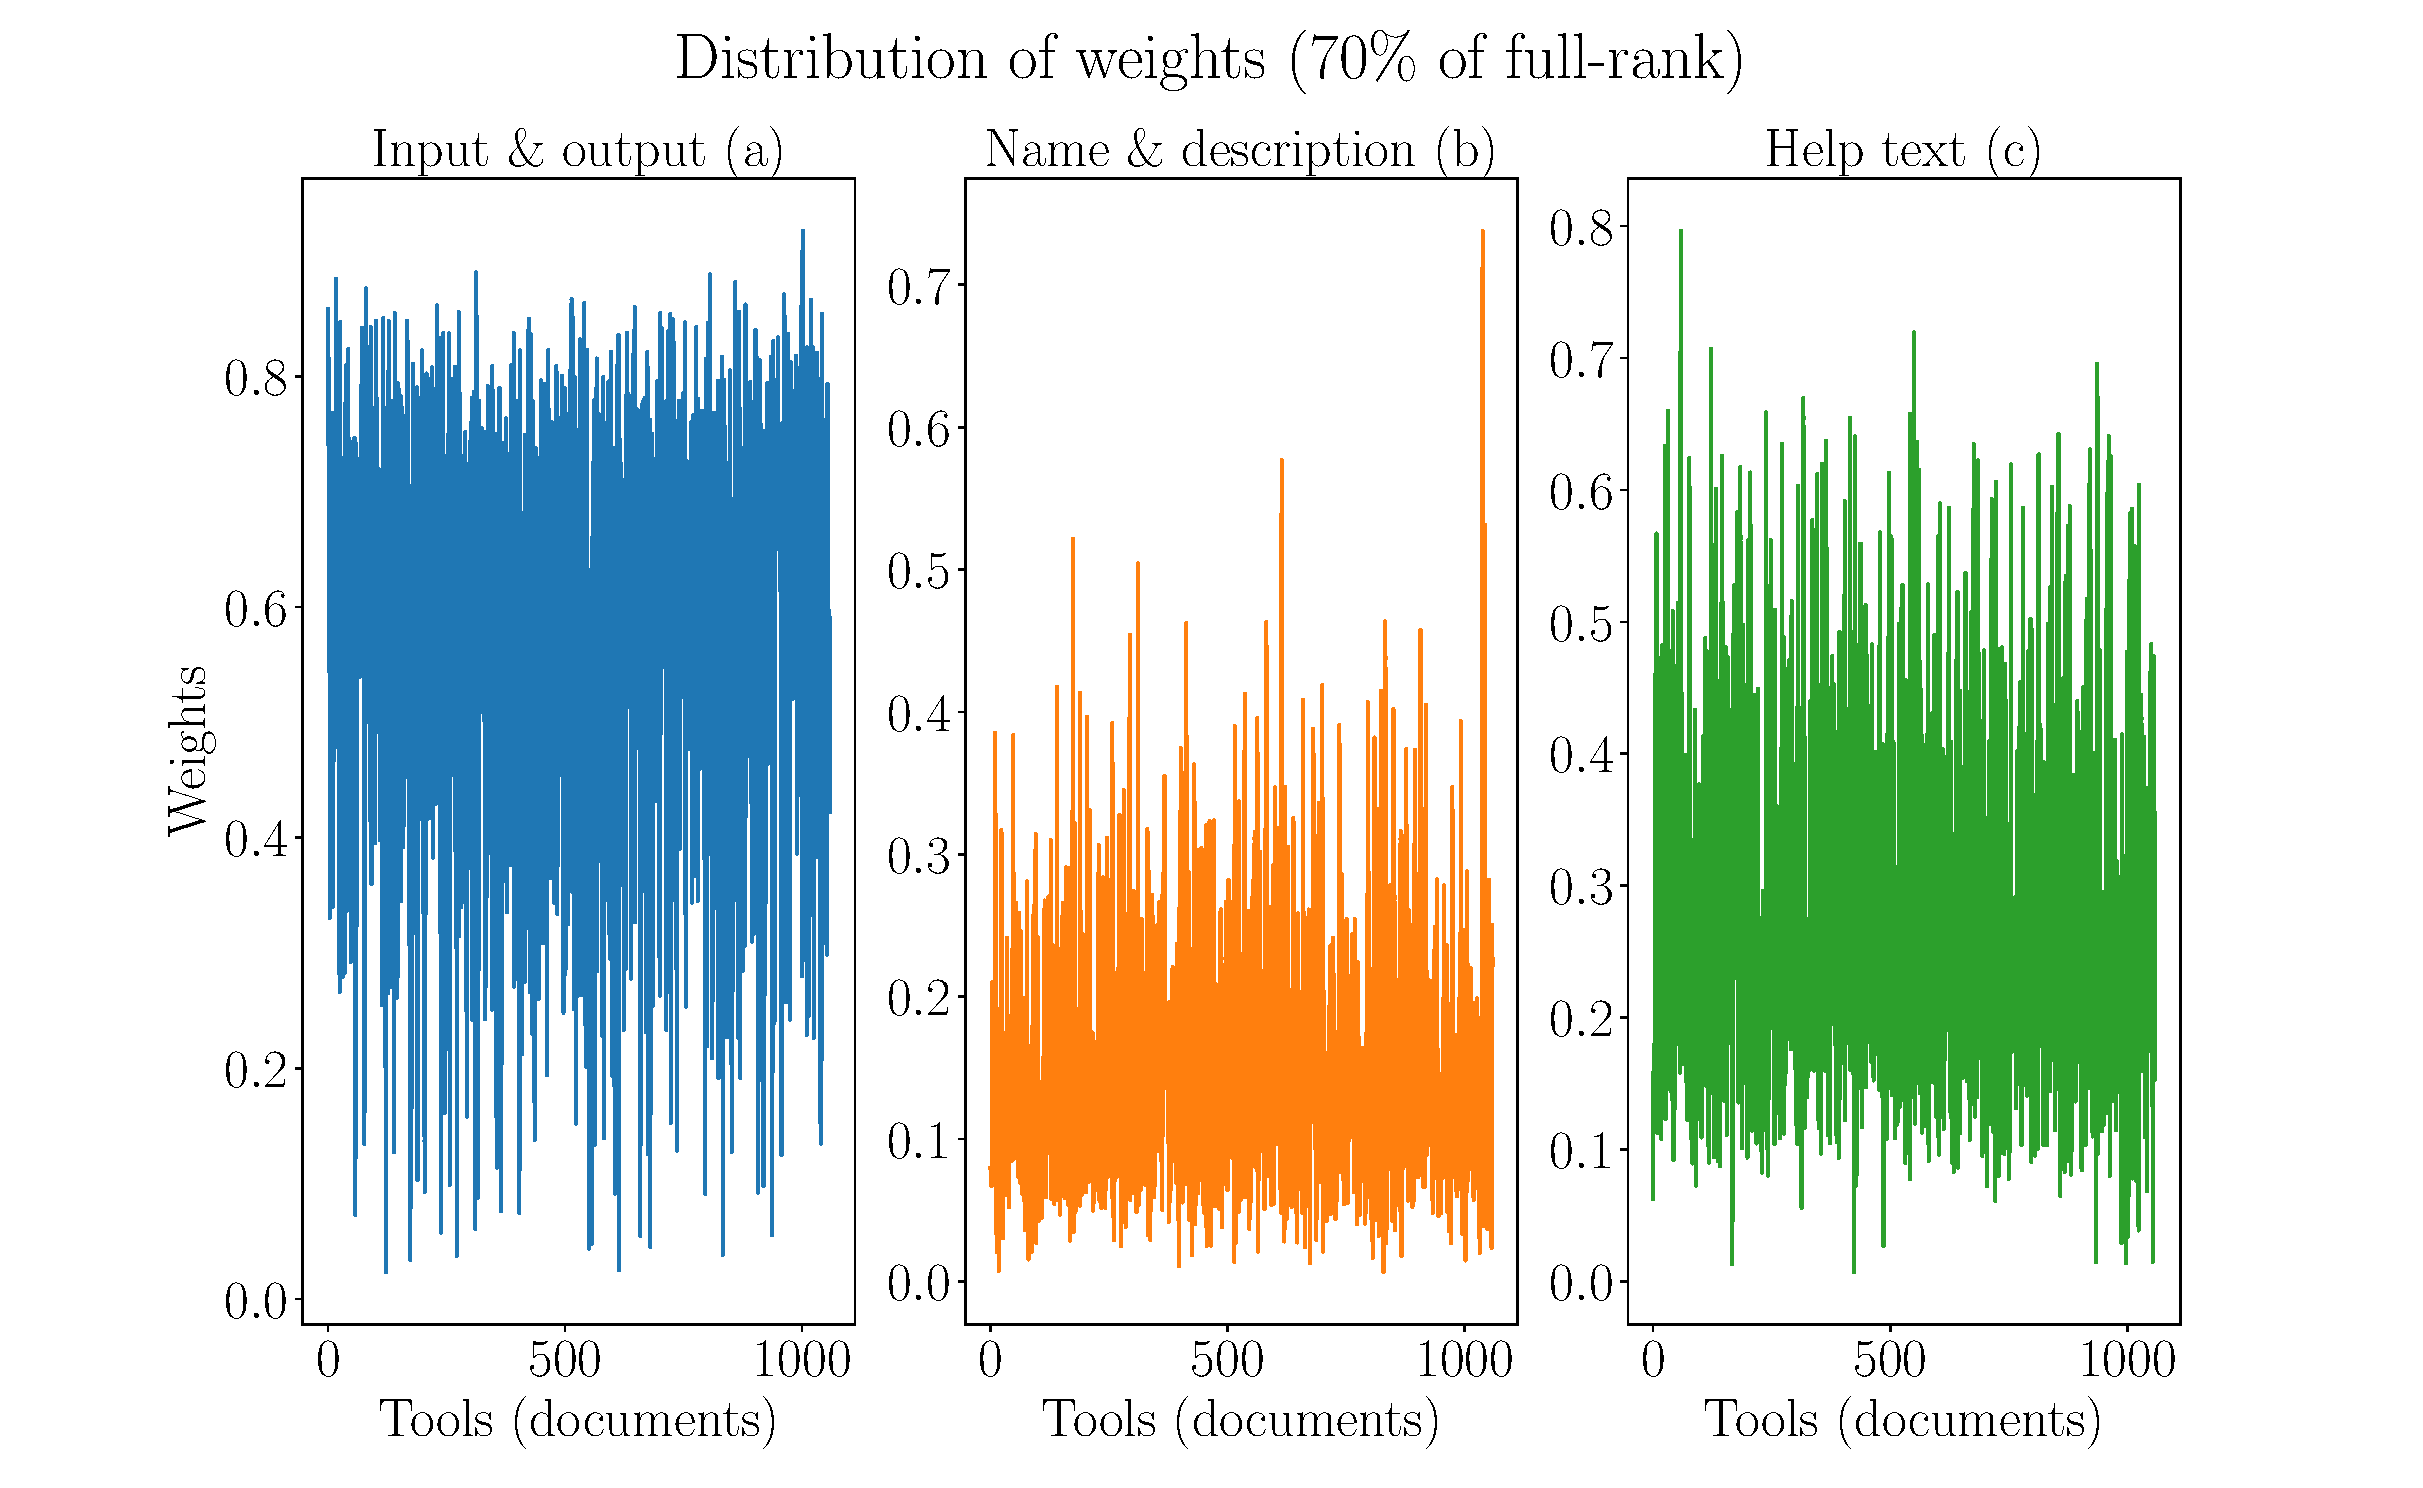
\includegraphics[scale=0.35]{figures/Weights_070.pdf}}
    \caption[Weights distribution 70\% rank]{\textbf{Weights distribution using 70\% of full-rank}: The plot shows the distribution of weights learned by gradient descent optimizer on the similarity matrices for the input and output, name and description and help text attributes. The corresponding documents-tokens matrices contain 70\% of their full-ranks.}
\end{centering}
\end{figure}


\subsection{30\% of full-rank}
We reduce the ranks of two documents-tokens matrices to 30\% of the original ranks.

\begin{figure}[h]
\begin{centering}
    {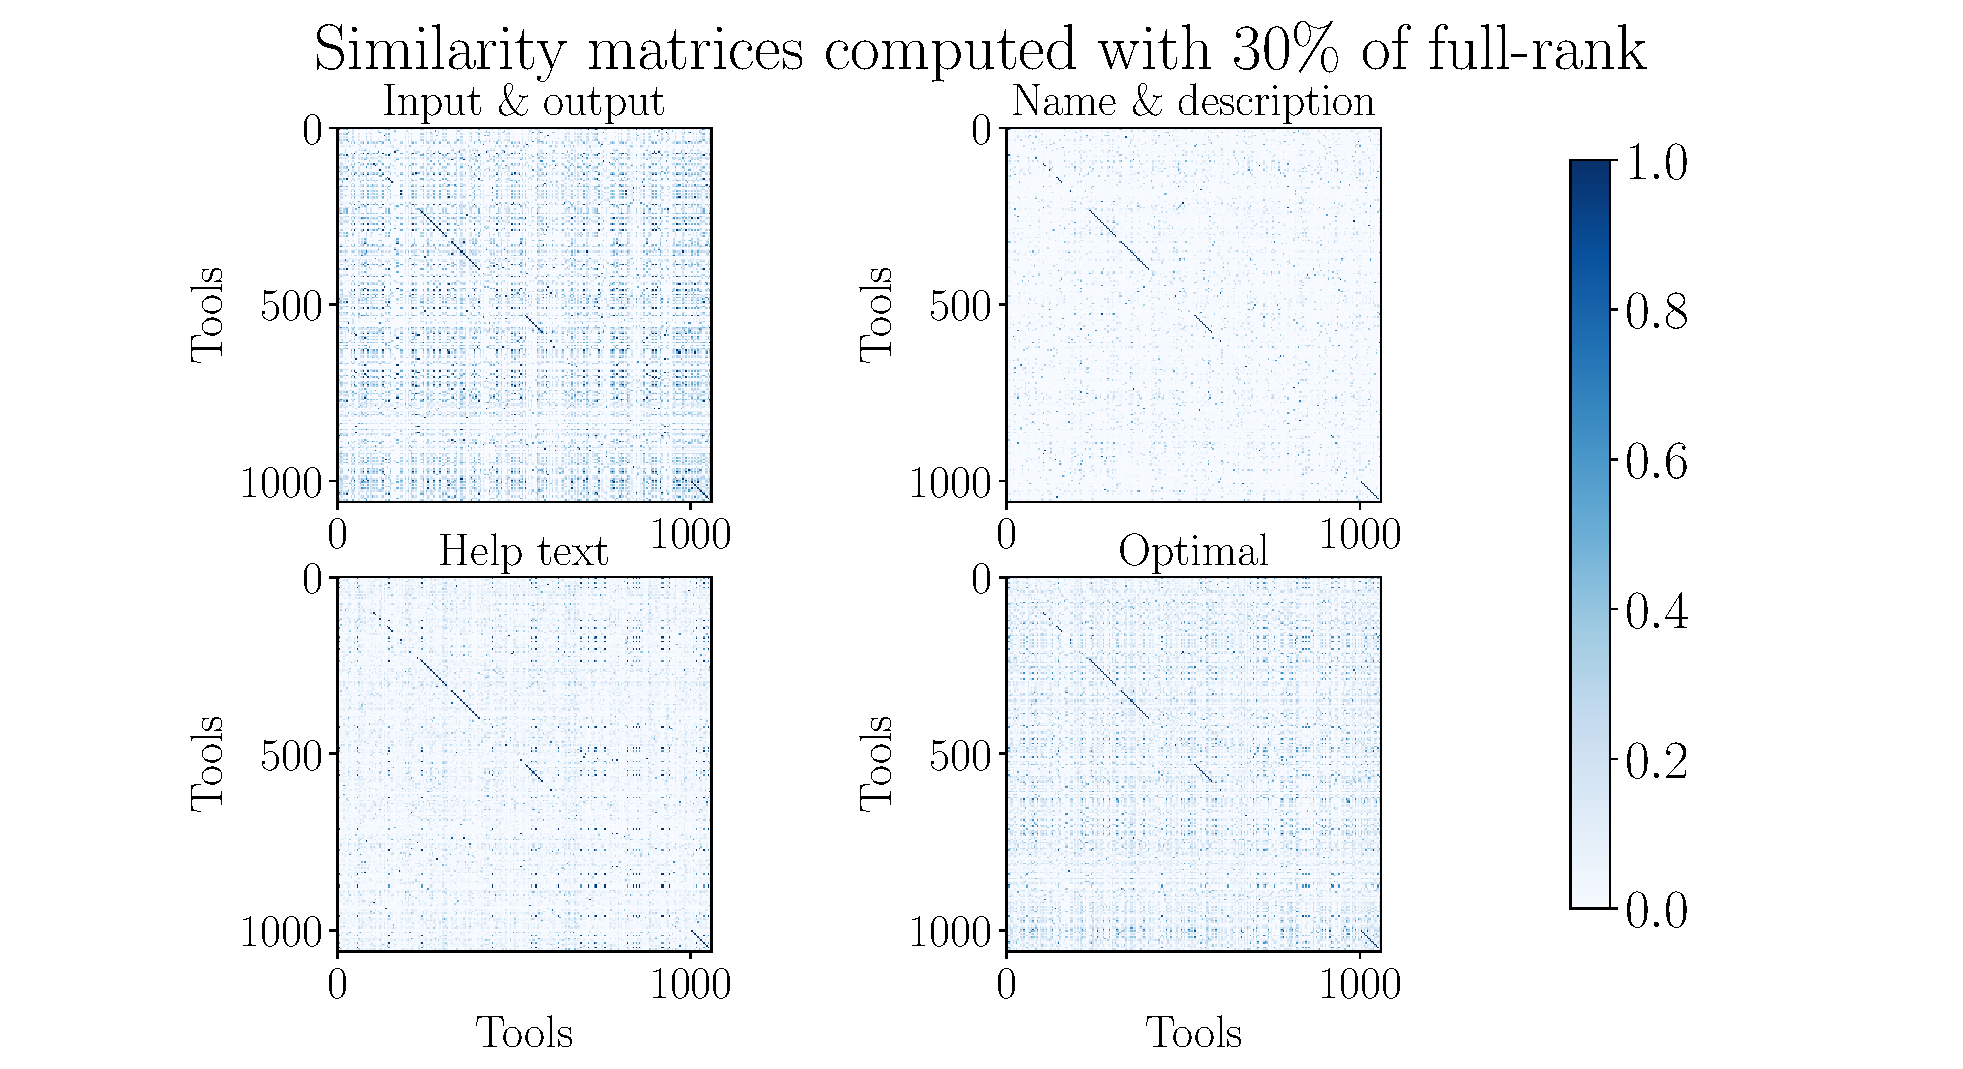
\includegraphics[scale=0.35]{figures/Similarity_matrices_030.pdf}}
    \caption[Similarity matrices 30\% rank]{\textbf{Similarity matrices using 30\% of full-rank}: The heatmap shows documents-documents (tools-tools) correlation matrices for input and output (a), name and description (b) and help text (c) attributes. The (d) shows a documents-documents (tools-tools) correlation matrix which is the weighted average computed using (a), (b) and (c) and weights (figure 22) given by the gradient descent optimizer (equation 15). The corresponding documents-tokens matrices are reduced to 30\% of their respective full-ranks.}
\end{centering}
\end{figure}

\begin{figure}[h]
\begin{centering}
    {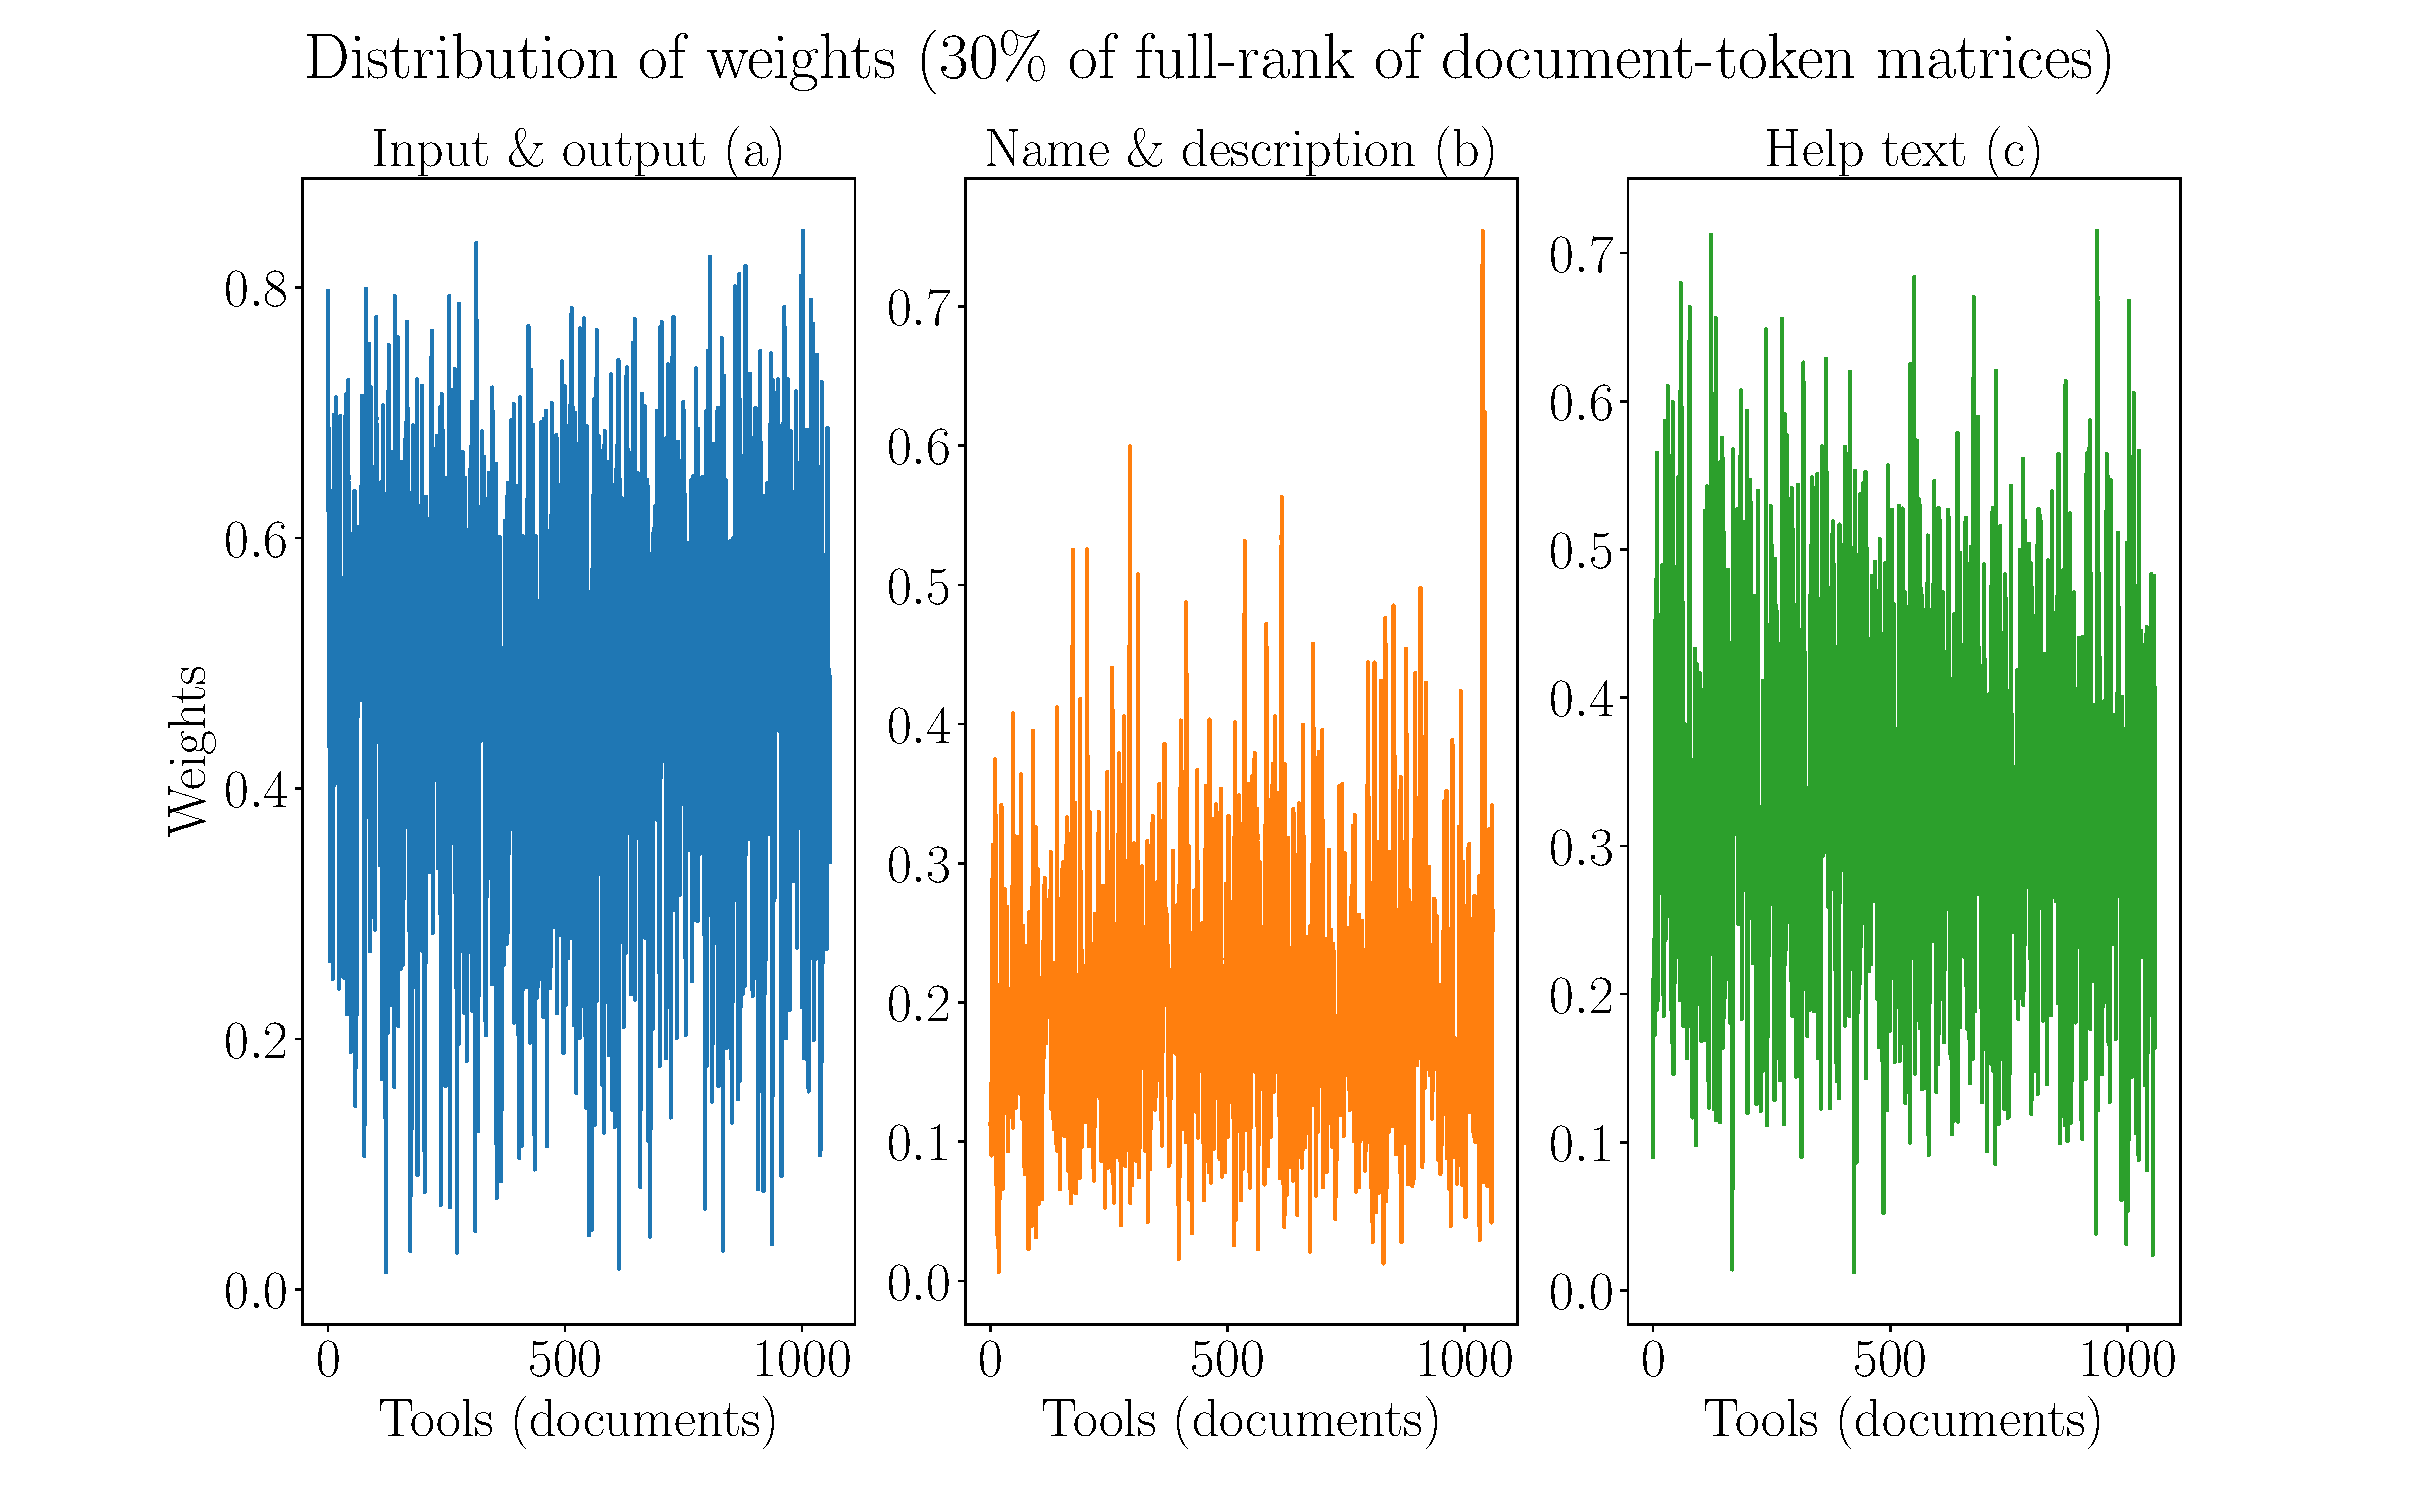
\includegraphics[scale=0.35]{figures/Weights_030.pdf}}
    \caption[Weights distribution 30\% rank]{\textbf{Weights distribution using 30\% of full-rank}: The plot shows the distribution of weights learned by gradient descent optimizer on the similarity matrices for the input and output, name and description and help text attributes. The corresponding documents-tokens matrices contain 30\% of their full-ranks.}
\end{centering}
\end{figure}

\subsection{5\% of full-rank}
We reduce the ranks of two documents-tokens matrices to 5\% of the original ranks.

\begin{figure}[h]
\begin{centering}
    {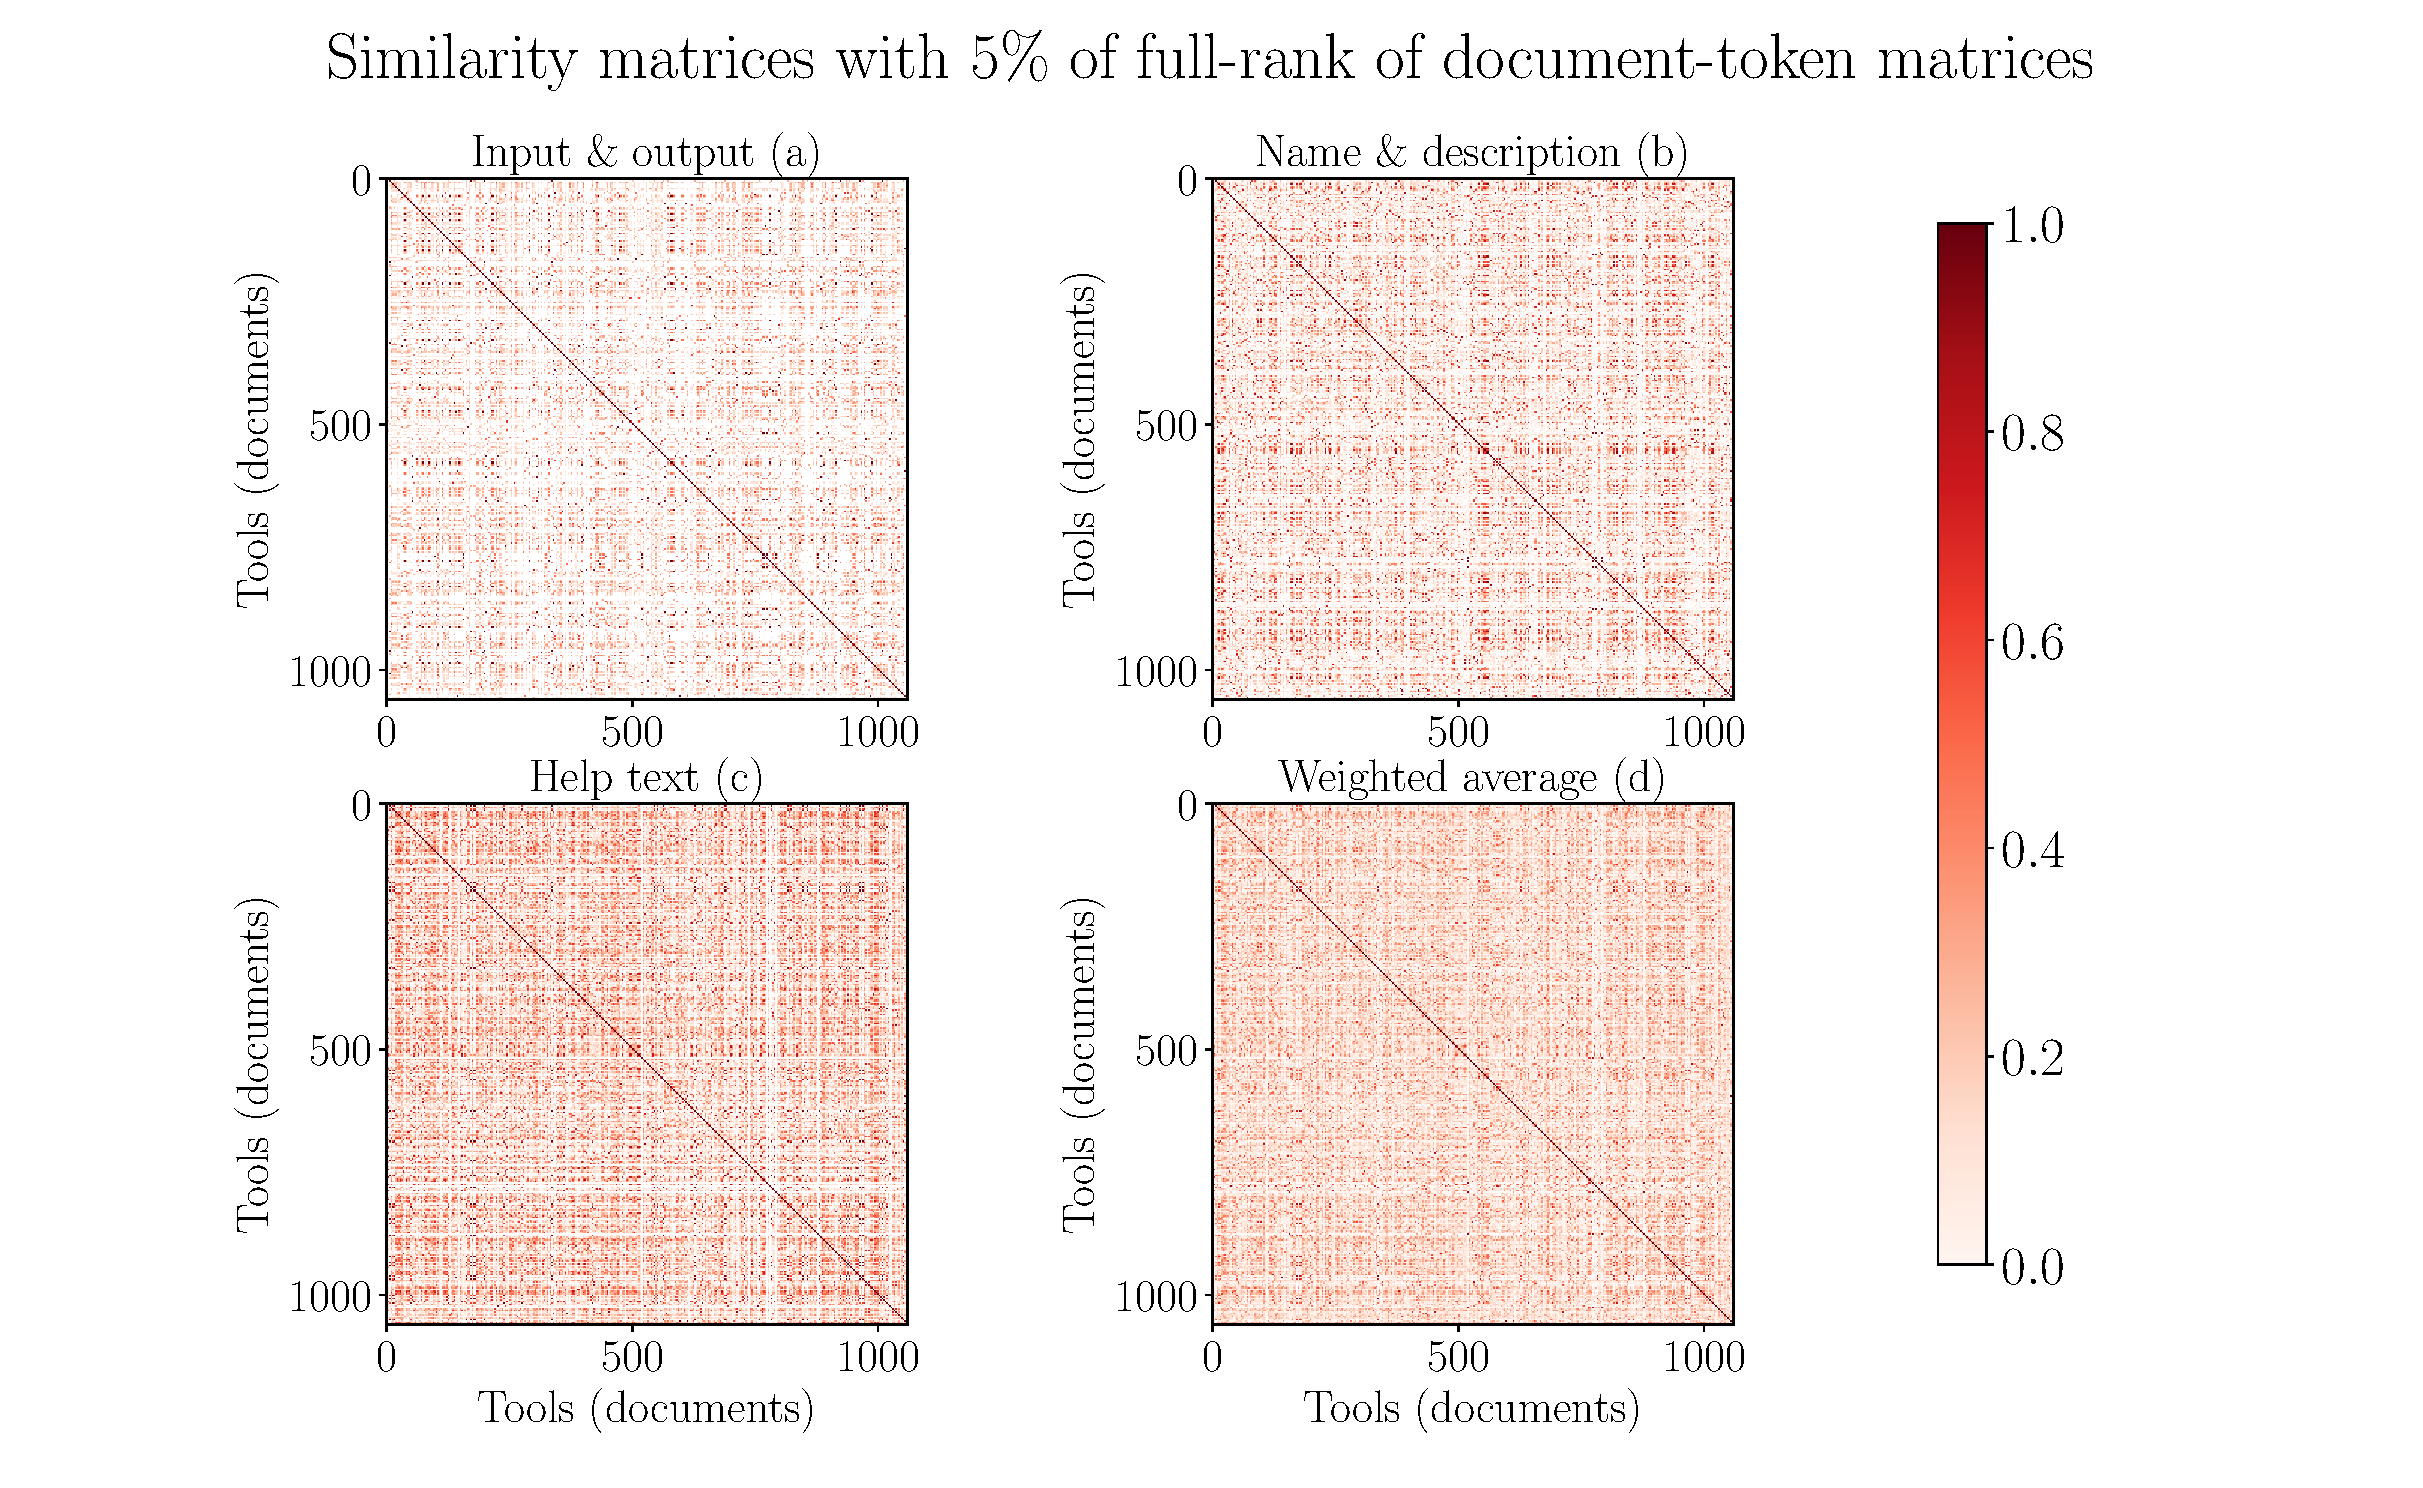
\includegraphics[scale=0.35]{figures/Similarity_matrices_005.pdf}}
    \caption[Similarity matrices 5\% rank]{\textbf{Similarity matrices using 5\% of full-rank}: The heatmap shows documents-documents (tools-tools) correlation matrices for input and output (a), name and description (b) and help text (c) attributes. The (d) shows a documents-documents (tools-tools) correlation matrix which is the weighted average computed using (a), (b) and (c) and weights (figure 24) given by the gradient descent optimizer (equation 15). The corresponding documents-tokens matrices are reduced to 5\% of their respective full-ranks.}
\end{centering}
\end{figure}

\begin{figure}[h]
\begin{centering}
    {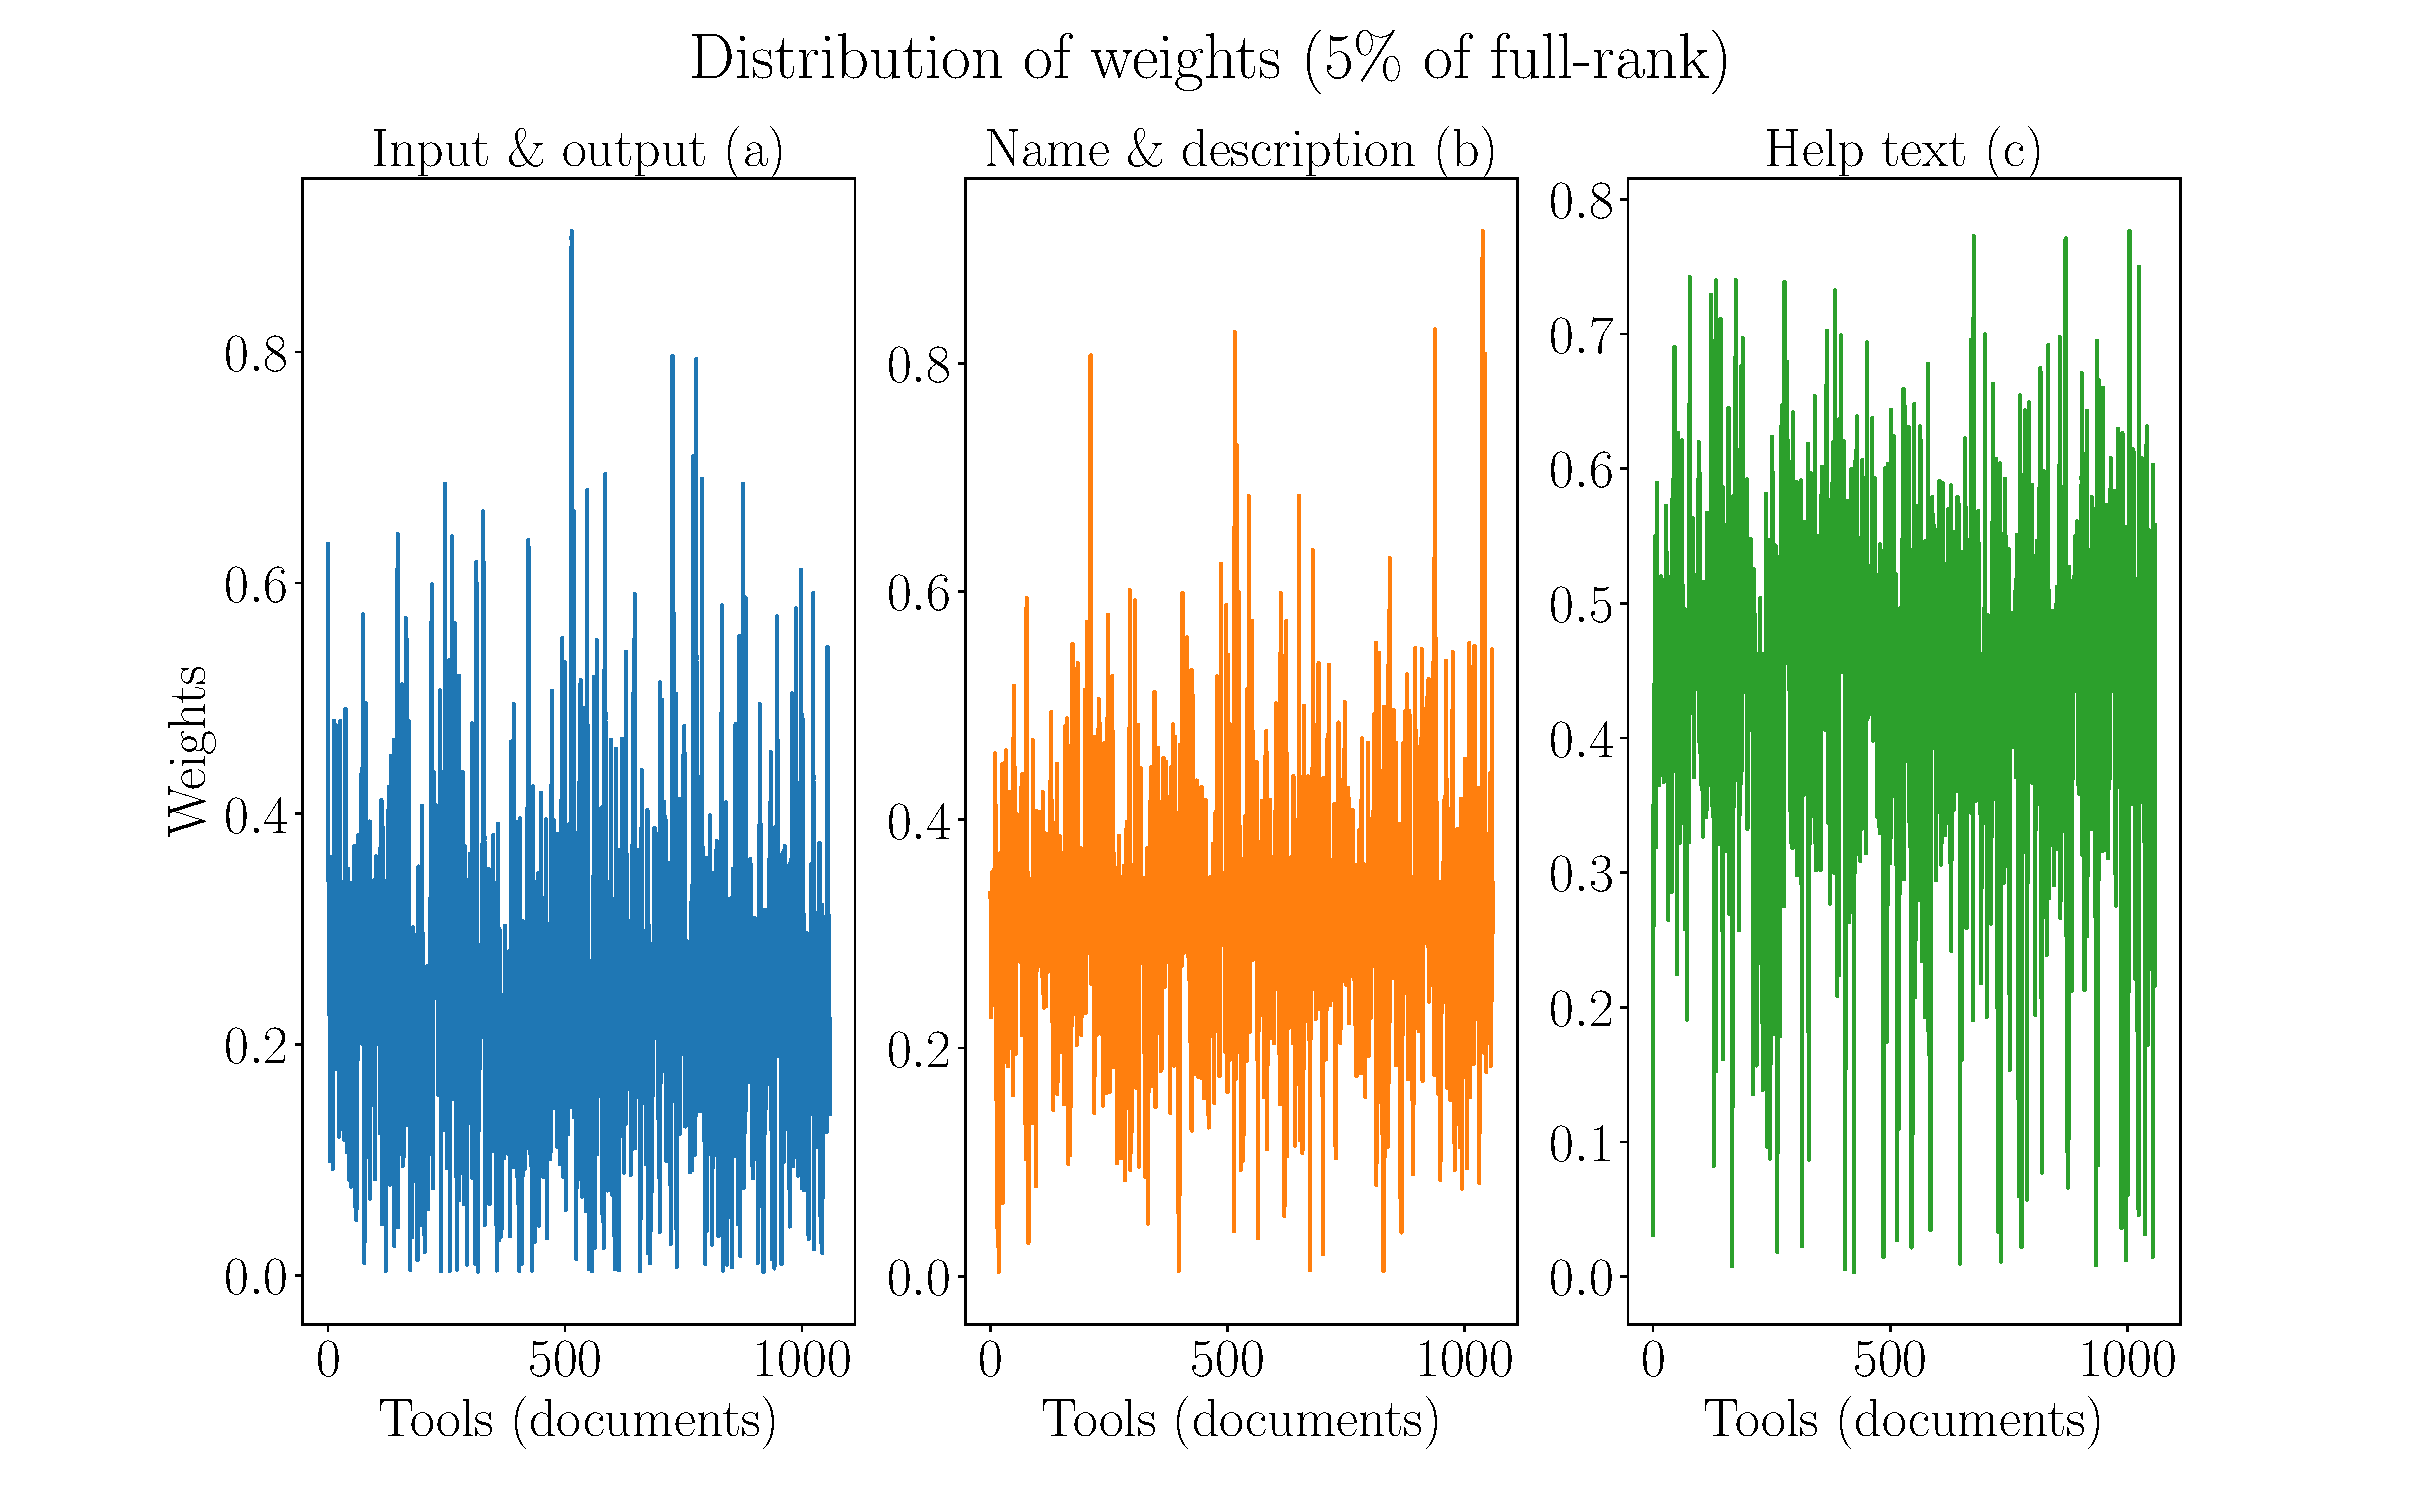
\includegraphics[scale=0.35]{figures/Weights_005.pdf}}
    \caption[Weights distribution 5\% rank]{\textbf{Weights distribution using 5\% of full-rank}: The plot shows the distribution of weights learned by gradient descent optimizer on the similarity matrices for the input and output, name and description and help text attributes. The corresponding documents-tokens matrices contain 5\% of their full-ranks.}
\end{centering}
\end{figure}

\subsection{Reduction in error}
We observe the loss in mean squared error when we decrease the ranks of the matrices. When we reduced the ranks, the similarity scores for the name and description and help text increase. This increase accounts for their higher importance weights learnt by the optimizer. The importance weights on an average become more balanced and can account for the decrease in the mean squared error. We would also see that in the next section that the ranking of similar tools also become better after rank reduction.

\begin{figure}[h]
\begin{centering}
    {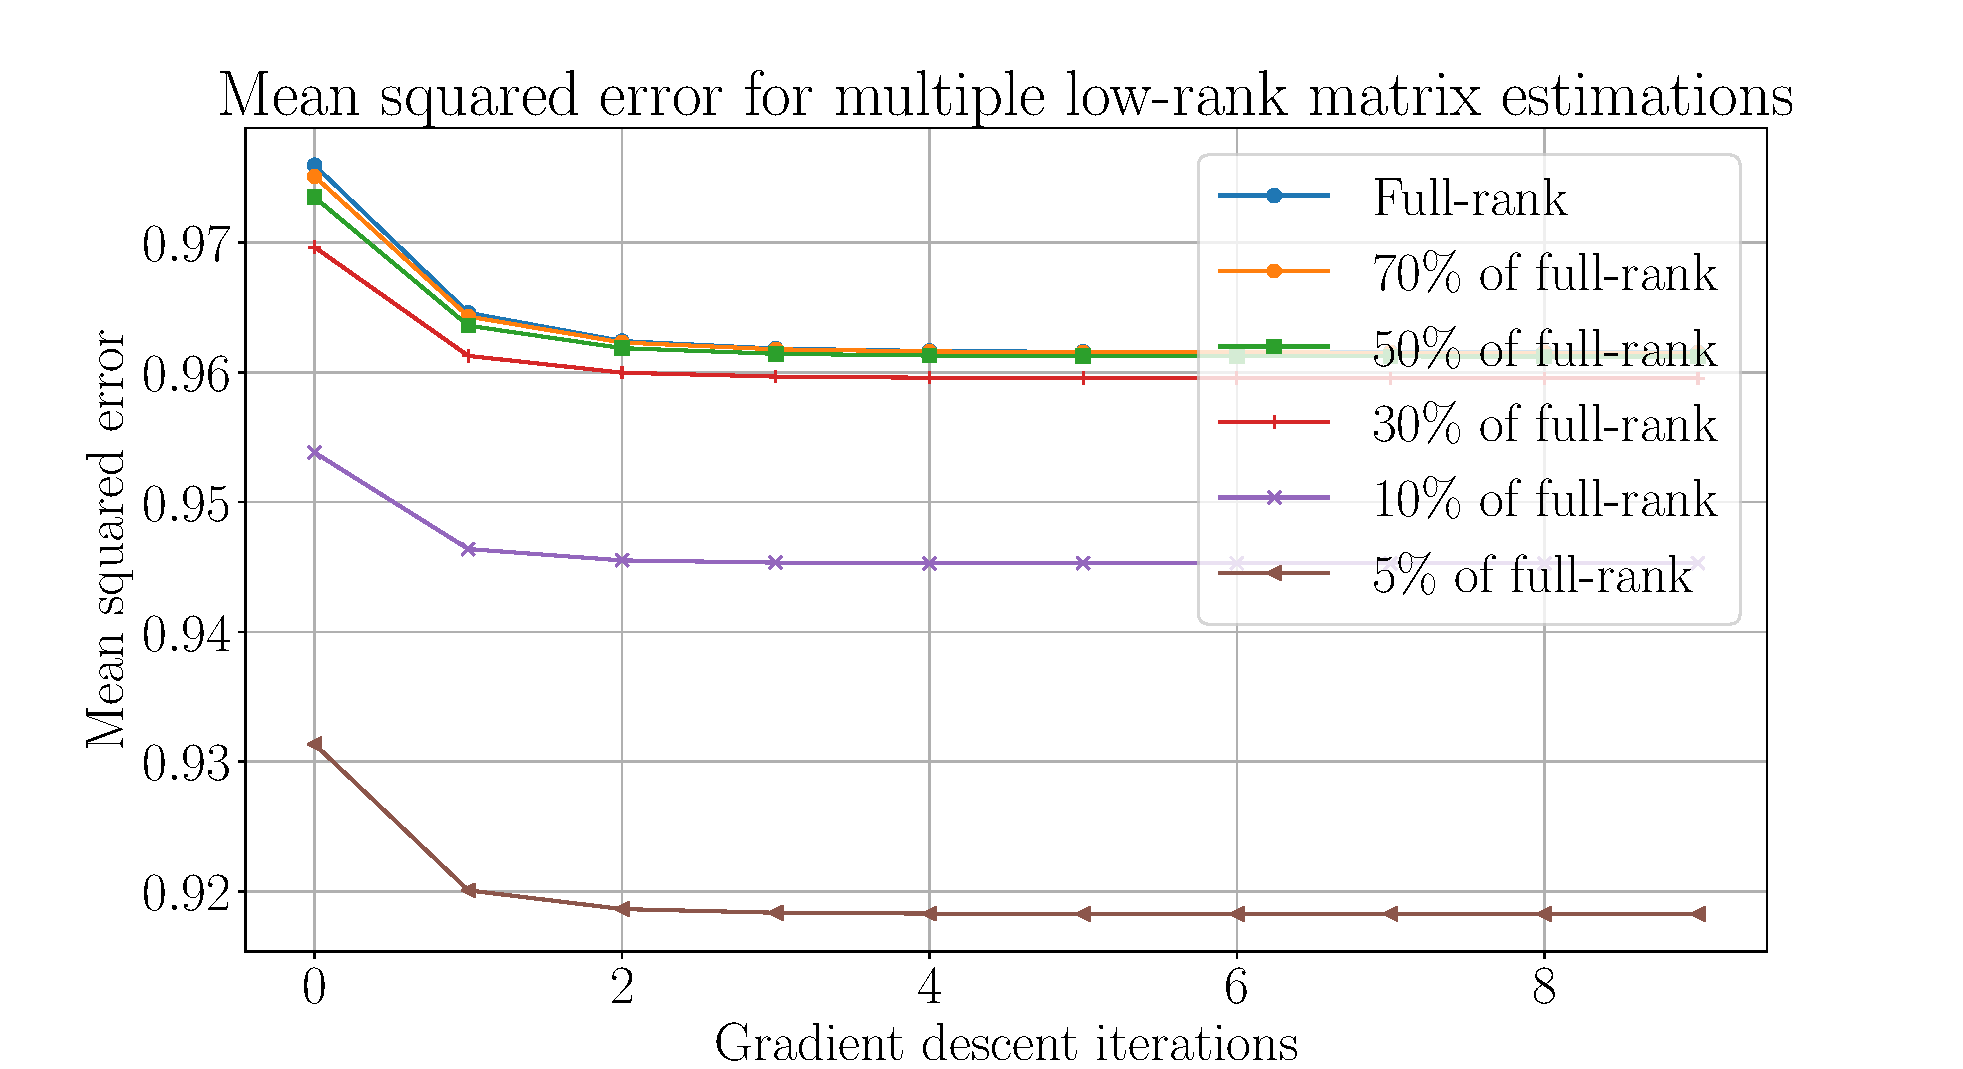
\includegraphics[scale=0.35]{figures/MSE_iterations_low_rank.pdf}}
    \caption[Mean squared error using LSI]{\textbf{Mean squared error using full-rank and multiple estimations of low-rank documents-tokens matrices}: This shows an mean squared error comparison computed using full-rank and various estimations of low-rank documents-tokens matrices. Each line plot shows an average error over all the tools and attributes which drops as we move along the iterations of gradient descent.}
\end{centering}
\end{figure}

\section{Paragraph vectors}

\begin{figure}[h]
\begin{centering}
    {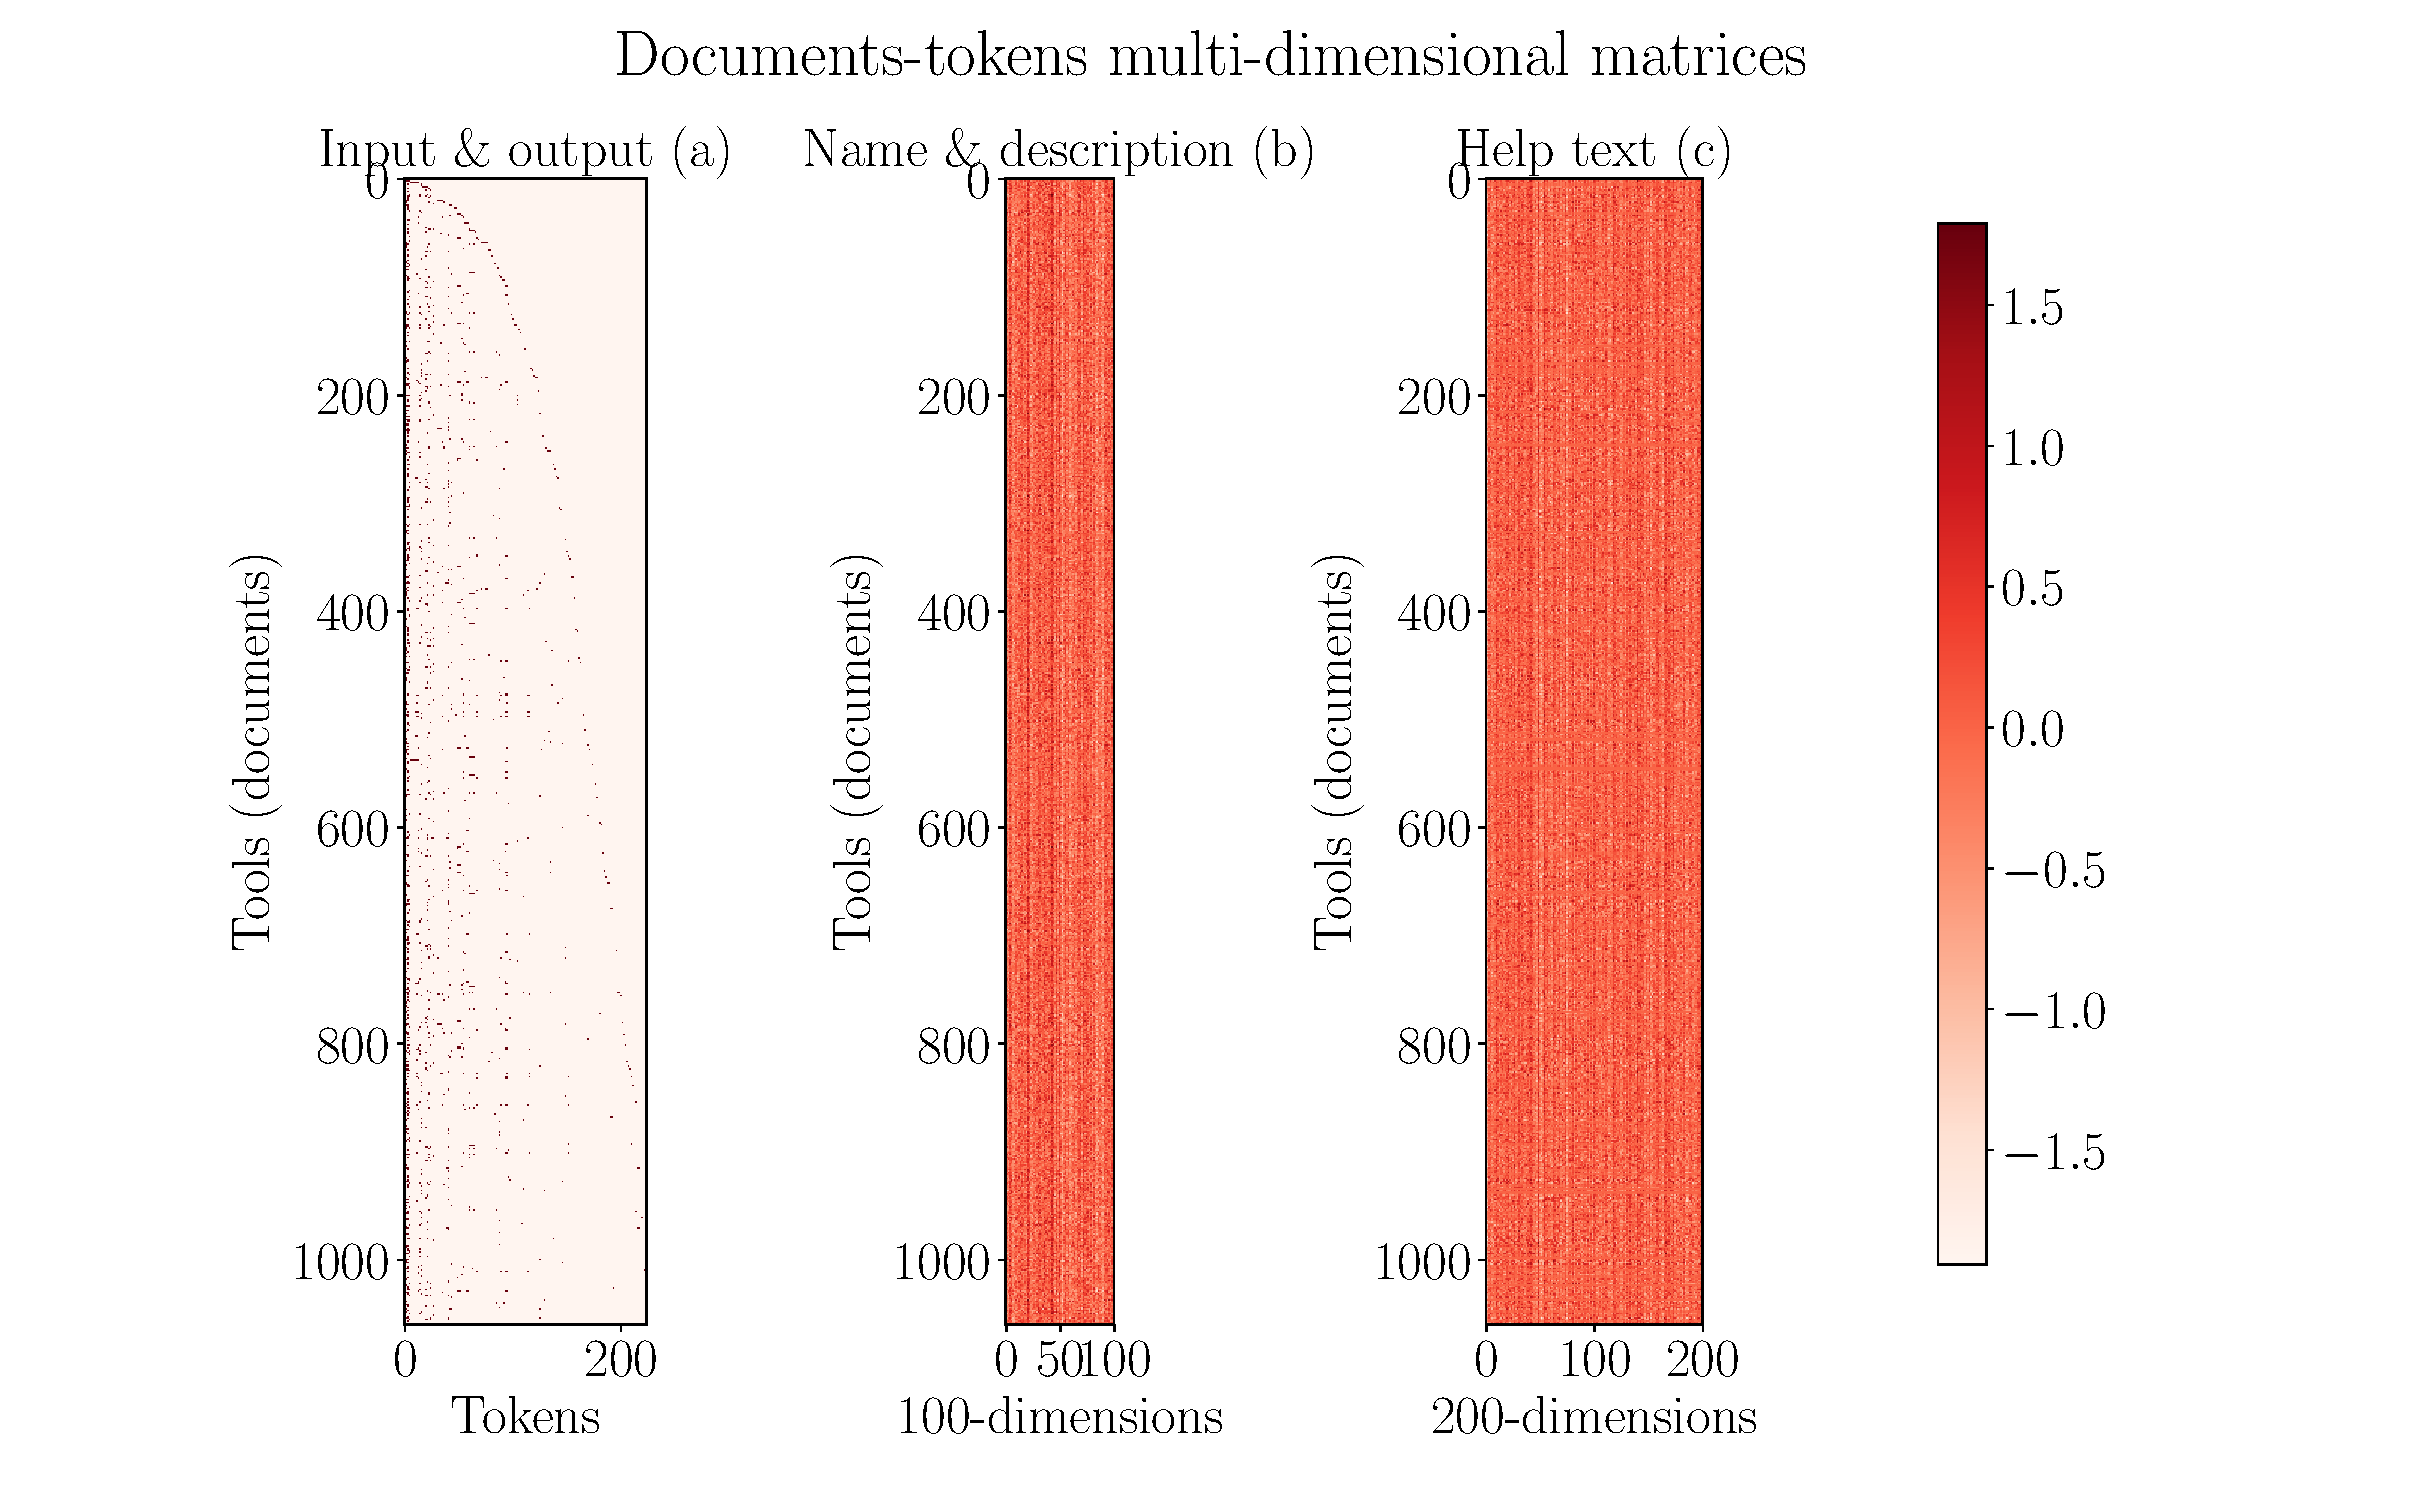
\includegraphics[scale=0.35]{figures/Documents-tokens_doc2vec.pdf}}
    \caption[Documents-tokens matrices for paragraph vectors]{\textbf{Documents-tokens matrices for paragraph vectors approach}: The heatmap shows documents-tokens matrices for input and output file types (a), name and description (b) and help text (c) attributes. The matrix in (a) is a document-token matrix where each entry shows a relative frequency of the token's occurrence. The matrices in (b) and (c) are 100 and 200 dimensional (each row is a document vector) respectively which means that each row of a matrix belongs to a document (paragraph) and is fixed-length and dense in nature. }
\end{centering}
\end{figure}

\begin{figure}[h]
\begin{centering}    
    {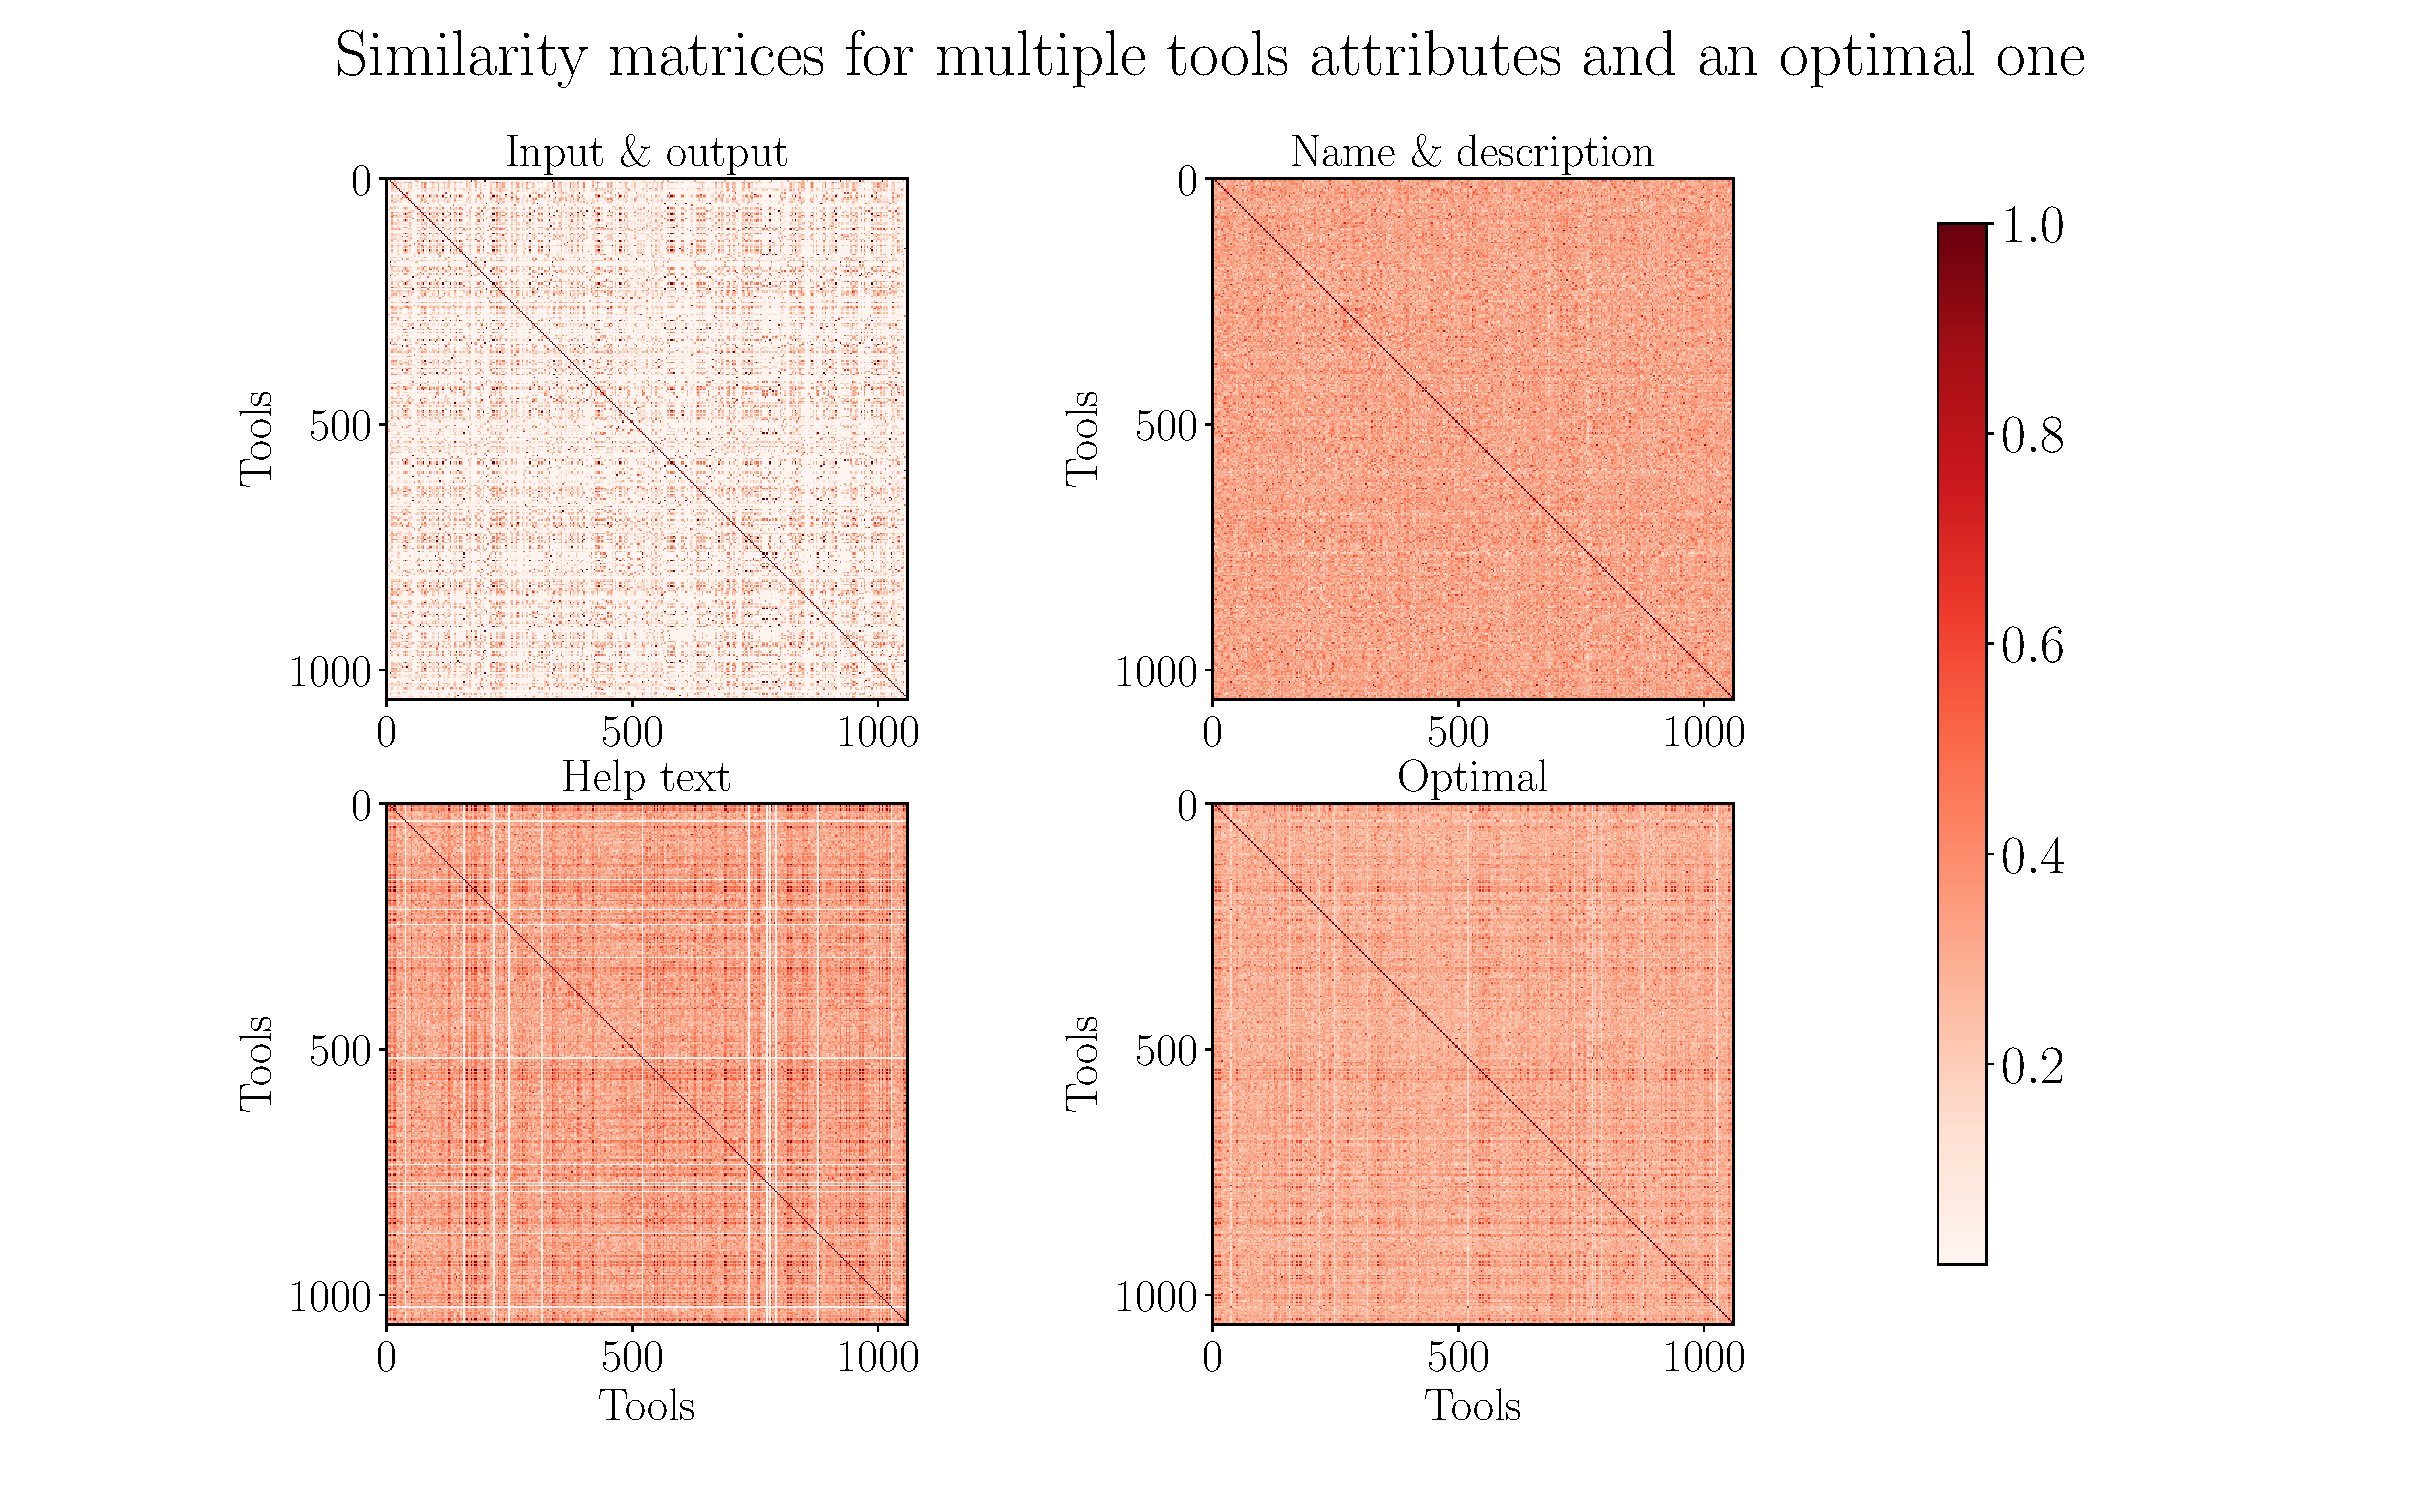
\includegraphics[scale=0.35]{figures/Similarity_matrices_doc2vec.pdf}}
    \caption[Similarity matrices using paragraph vectors approach]{\textbf{Similarity matrices using paragraph vectors approach}: The heatmap shows documents-documents (tools-tools) correlation matrices for input and output (a), name and description (b) and help text (c) attributes. The (d) shows a documents-documents (tools-tools) correlation matrix which is the weighted average computed using (a), (b) and (c) and weights (figure 22) given by the gradient descent optimizer (equation 15). The corresponding documents-tokens matrices are computed as shown in figure 26.}
\end{centering}
\end{figure}

\begin{figure}[h]
\begin{centering}
    {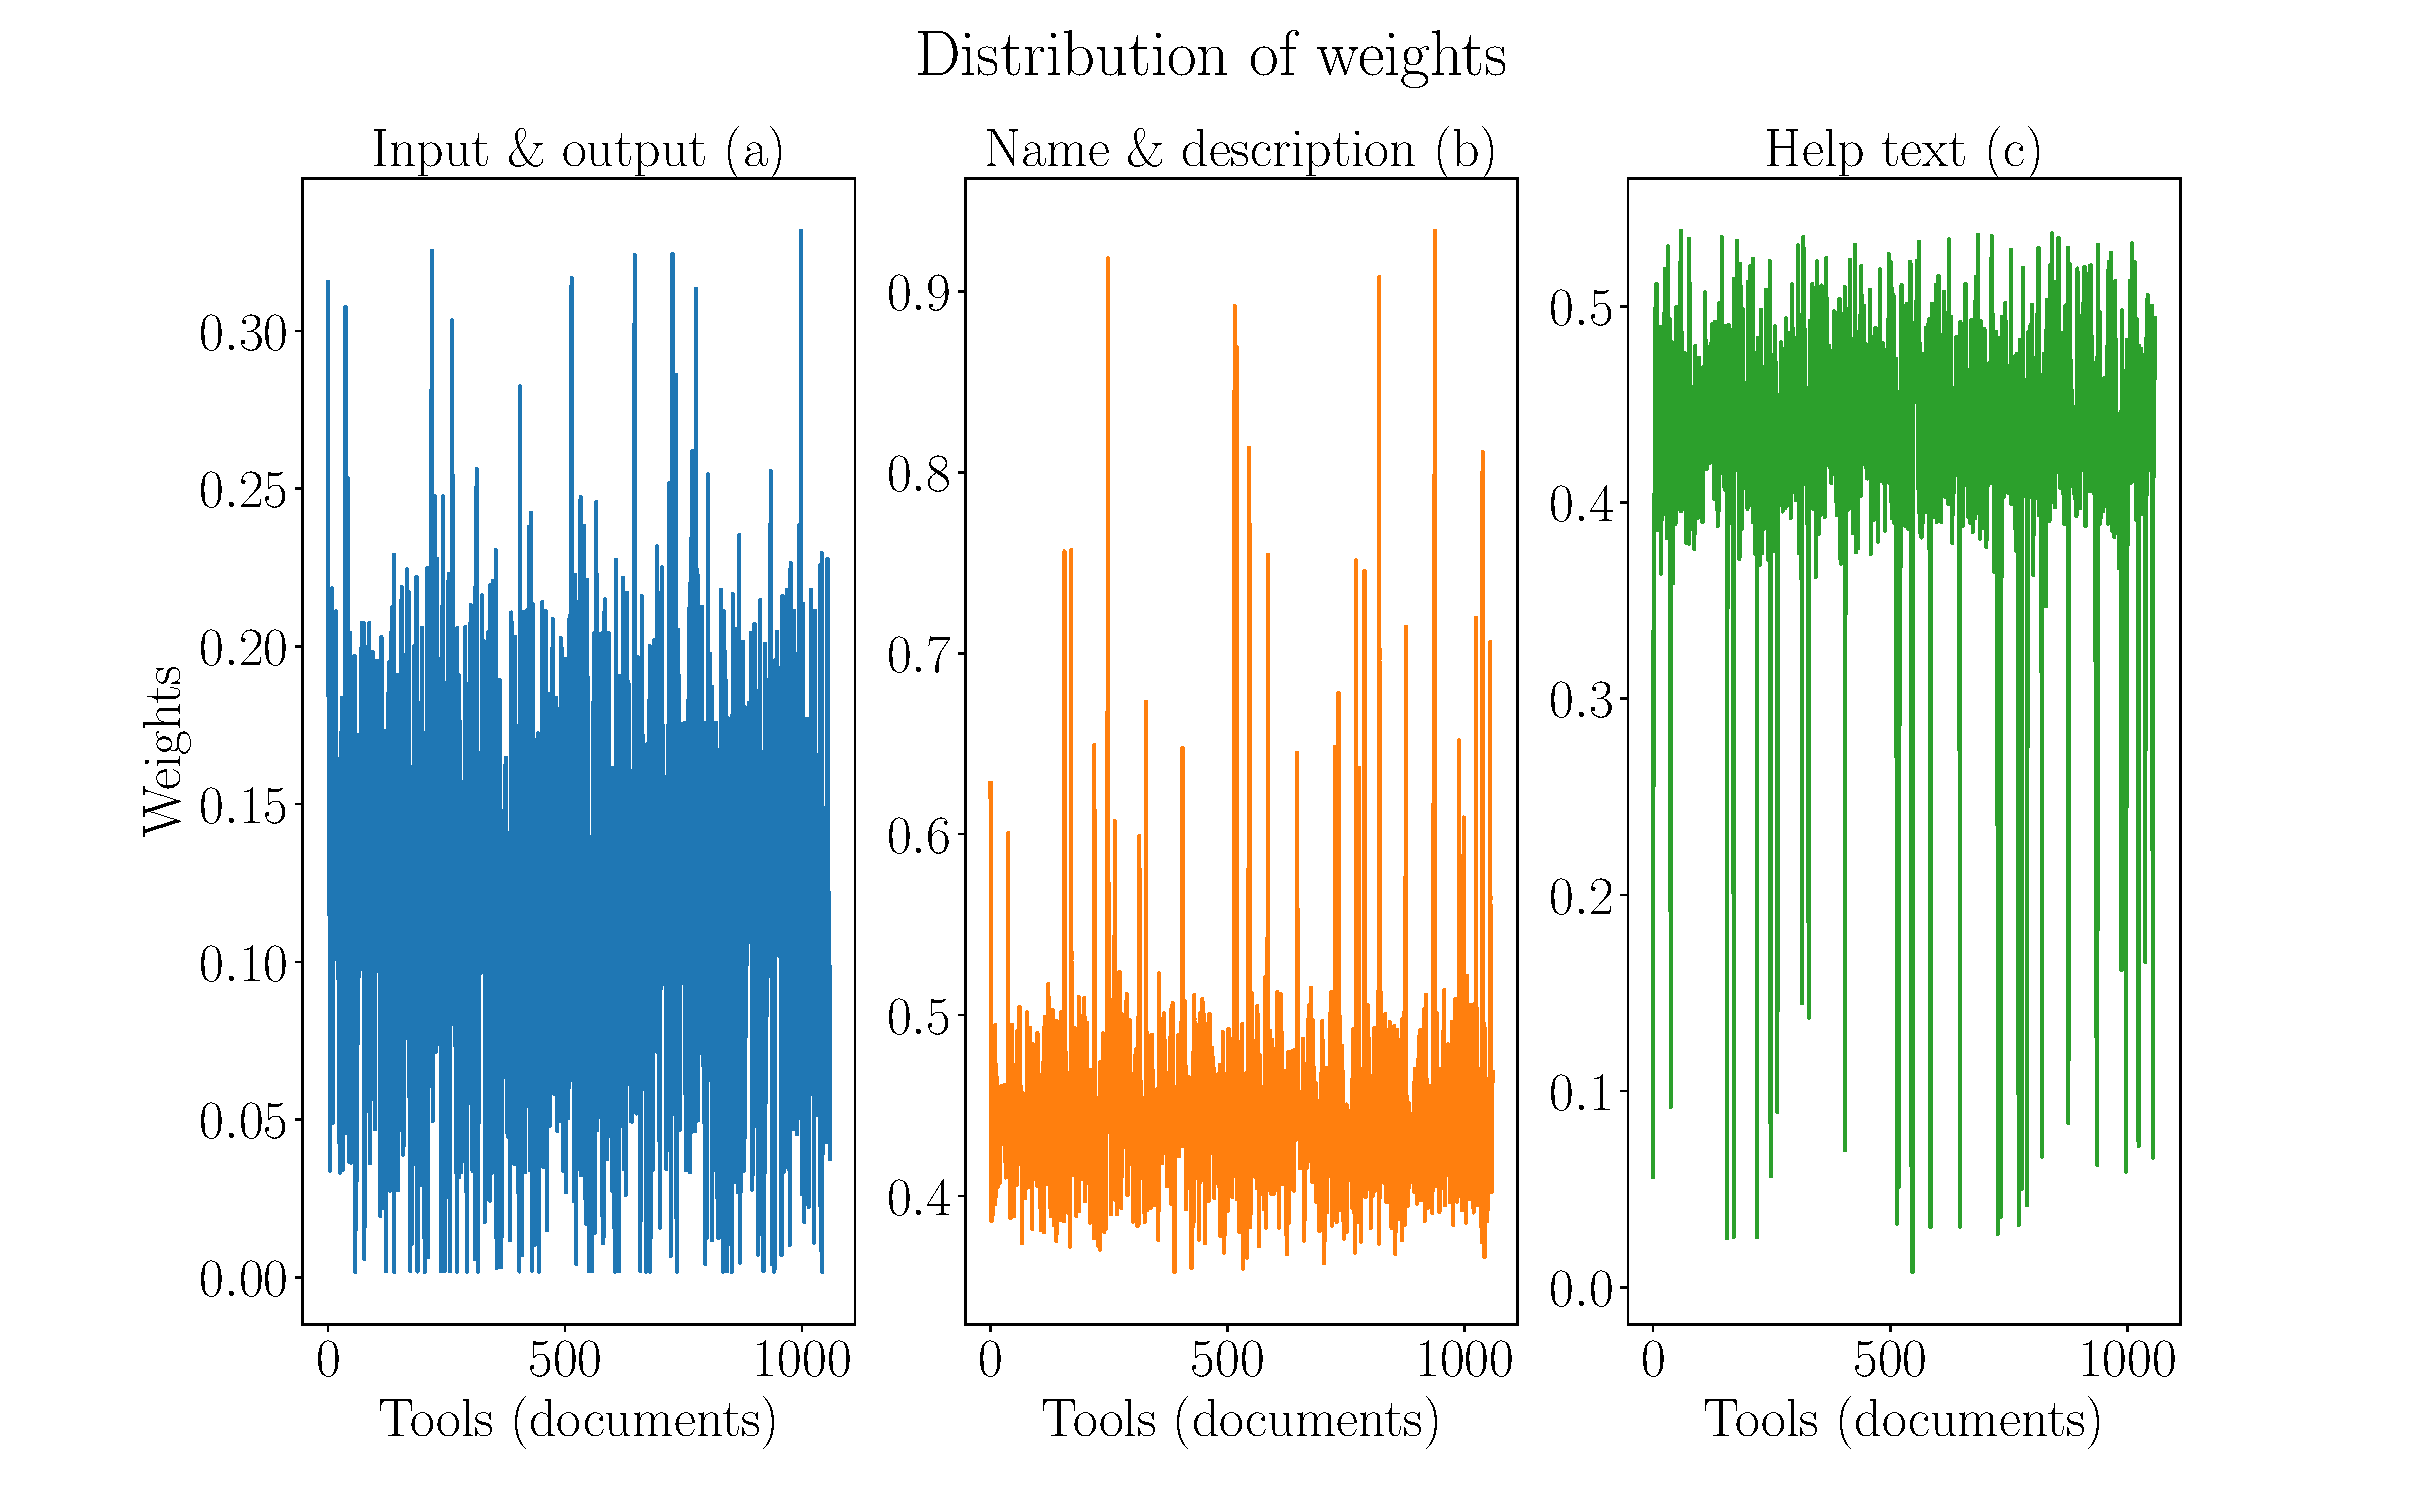
\includegraphics[scale=0.35]{figures/Weights_doc2vec.pdf}}
    \caption[Weights distribution for doc2vec]{\textbf{Weight distribution learnt using paragraph vectors approach}: The plot shows the distribution of weights learned by gradient descent optimizer on the similarity matrices for the input and output (a), name and description (b) and help text (c) attributes. The corresponding documents-tokens matrices are computed as shown in figure 26. }
\end{centering}
\end{figure}


\subsection{Learning rate}


\subsection{Visualizer}
\subsection{LSI}
\subsection{Paragraph vectors}


